% By zmienic jezyk na angielski/polski, dodaj opcje do klasy english lub polish
\documentclass[polish,12pt]{aghthesis}
\usepackage[utf8]{inputenc}
\usepackage[usenames, dvipsnames]{color}
\usepackage{hyperref}
\usepackage{titlesec}
\usepackage{wrapfig}
\usepackage{lipsum}
\usepackage{float}
\usepackage{caption}

\setcounter{secnumdepth}{4}

\author{Wojciech Karpiel\\ Michał Hamuda\\ Filip Galas}

\titlePL{System rejestracji pacjentów - PRZEMEK}
\titleEN{Patient registration system}

\fieldofstudy{Informatyka}

\supervisor{dr inż. Bartłomiej Śnieżyński}

\date{2017}

% Szablon przystosowany jest do druku dwustronnego, 
\begin{document}

\maketitle

\tableofcontents

\newpage

\section{Cel prac i wizja produktu}
%\section{Project goals and vision}
\label{sec:cel-wizja}

Poniżej znajduje się opis problemu który produkt rozwiązuje, celu produktu, analiza potencjalnych problemów przy tworzeniu produktu.
  
\subsection{Opis problemu}
Jednym z głównych zadań gabinetu lekarskiego jest przyjmowanie pacjentów na wizyty u lekarza. Zanim pacjent będzie mógł odbyć wizytę, zazwyczaj konieczna jest jego rejestracja. W ogólnym przypadku może ona przebiegać według poniższych kroków:

\begin{enumerate}
  \item Pacjent znajduje numer telefonu do recepcji gabinetu.
  \item Pacjent dzwoni do recepcji gabinetu.
  \item Recepcjonistka odbiera telefon.
  \item Pacjent przedstawia cel wizyty bądź nazwisko lekarza.
  \item Recepcjonistka odszukuje w grafiku możliwe terminy wizyty.
  \item Recepcjonistka podaje pacjentowi możliwe terminy wizyty.
  \item Pacjent wybiera termin wizyty.
  \item Recepcjonistka wpisuje termin do grafiku lekarza.
  \item Pacjent wpisuje termin do swojego kalendarza.
\end{enumerate}

W powyższym modelu wyróżniamy następujące niedogodności i problemy:
\begin{itemize}
%todo tu można jeszcze więcej głupot napisać
  \item Potrzeba znalezienia przez pacjenta numeru telefonu do gabinetu.
  \item Konieczność stałej obsługi linii telefonicznej przez recepcjonistkę w godzinach, w których pacjent ma możliwość rejestracji.
  \item Konieczność prowadzenia przez gabinet rejestru wizyt.
  \item Możliwość błędnego zapisania terminu lub zapomnienia przez pacjenta o umówionym terminie wizyty.
  \item Konieczność powiadomienia lekarza o nowej rezerwacji terminu wizyty w sposób ustny bądź pisemny.
  \item Brak natychmiastowego dostępu przez lekarza do danych pacjenta.
\end{itemize}

\subsection{Cel}
Stworzyć system eliminujący podane wyżej problemy i niedogodności, a w szczególności:

\begin{itemize}
  \item Dostarczyć pacjentowi możliwość samodzielnej rejestracji na wizytę u lekarza.
  \item Dostarczyć pacjentowi widok kalendarza pozwalający na ogląd dostępnych terminów i ich wybór oraz ogląd terminów zarezerwowanych wizyt.
  \item Dostarczyć lekarzowi widok kalendarza pozwalający ustalić godziny przyjęć, oznaczyć określone terminy jako niedostępne, zobaczyć zajęte przez pacjentów terminy oraz odwołać wizyty.
  \item Ułatwić lekarzowi dostęp do danych medycznych pacjenta zapisanego na wizytę.
  \item Dostarczyć recepcjonistce widok kalendarza pozwalający na sprawne poinformowanie rejestrującego się pacjenta o dostępnych terminach oraz zapisać go na wizytę.
  \item Umożliwić wpisywanie danych osobowych oraz wypełnianie formularzy medycznych przez rejestrującego się pacjenta bądź przez recepcjonistkę pozyskującą dane od pacjenta.
  \item Umożliwić automatyczne gromadzenie danych związanych z wizytami.
\end{itemize}

\subsection{Motywacja}
Motywacją była dla nas chęć zdobycia wiedzy z zakresu wytwarzania oprogramowania dla potrzeb medycznych, poznania specyfiki tej dziedziny, a także nauczenia się efektywnego wykorzystywania technologii używanych przez nas w procesie tworzenia produktu końcowego. Ponadto, jest to praca dyplomowa, na podstawie której dążymy do uzyskania tytułu inżyniera.

\subsection{Wizja produktu}
Rozwiązaniem wymienionych wyżej problemów będzie aplikacja, do której użytkownicy będą mieli dostęp poprzez przeglądarkę internetową.

Aplikacja będzie rozróżniała trzy typy użytkowników:
\begin{itemize}
    \item Lekarz,
    \item Recepcjonistka,
    \item Pacjent.
\end{itemize}

Pacjent będzie mógł utworzyć swoje konto i zarejestrować się na wybrany termin wizyty spośród dostępnych terminów u wybranego lekarza. Recepcjonistka będzie mogła w imieniu pacjenta utworzyć jego konto i zarejestrować go na wizytę. Lekarz będzie mógł dodawać nowe terminy wizyt, przeglądać stan rezerwacji swoich wizyt i dane pacjentów

Szczegółowe możliwości wykorzystania systemu przez każdy typ użytkowników są opisane w \emph{wymaganiach funkcjonalnych}.

Wszystkie dane dot. pacjentów, lekarzy, dostępnych terminów wizyt i rezerwacji będą gromadzone w bazie danych.

\subsection{Studium wykonalności}
Technologie wymienione w \hyperref[subsec:analizaTechnologiczna]{\emph{Analizie technologicznej}} zostały uzgodnione przed rozpoczęciem prac z Klientem i pozostałymi zespołami --- było to konieczne ze względu na wysokie sprzężenie modułów przygotowywanych przez zespoły. Dlatego jesteśmy przekonani że technologie zostały dobrane poprawnie i produkt jest wykonalny ze względu na dobrane technologie.

Ograniczenia czasowe na wykonanie produktu zostały rozważone (miało to wpływ między innymi na \hyperref[subsec:wykorzystane-technologie-baza]{schemat bazy danych}).

Ponadto, przeprowadziliśmy analizę zagrożeń, której wyniki przedstawiamy poniżej.

\subsubsection{Analiza zagrożeń}
Możemy wyróżnić następujące czynniki ryzyka:
\begin{itemize}
  \item Rozbieżności między zespołami, a w szczególności:
  \begin{itemize}
    \item niespójna wizja produktu,
    \item niespójne API,
    \item porzucenie swojej części produktu lub niezrealizowanie wspólnych funkcjonalności przez którąkolwiek z zależnych grup.
  \end{itemize}
  Wszystkie wyżej wymienione zdarzenia uniemożliwiłyby powstanie w pełni działającego produktu, ze względu na to że poszczególne moduły są od siebie współzależne. Ryzyko wystąpienia rozbieżności można zminimalizować poprzez częste uzgadnianie między zespołami wizji produktu oraz API tych funkcjonalności, które udostępniane są zależnym modułom. Takie dyskusje powinny odbywać się nie tylko przed rozpoczęciem prac implementacyjnych, ale także w ich trakcie.
  \item Nieefektywne wykorzystanie technologii:
  \begin{itemize}
    \item front-endowych (\href{https://getbootstrap.com/}{Twitter Bootstrap}, \href{https://angular.io/}{Angular}),
    \item komunikacyjnych (HTTP API),
    \item zapewniających bezpieczeństwo (\href{https://jwt.io/}{JWT}).
  \end{itemize}
  Wyżej wymienione zdarzenia skutkowałyby powstaniem kosztownego w utrzymaniu lub niezapewniającego odpowiedniego poziomu bezpieczeństwa, lecz działającego produktu. Zapobieganie tego typu zagrożeniom polega na poznawaniu i stosowaniu najlepszych praktyk implementacji danej technologii.
  \item Utrata członka zespołu z przyczyn losowych, np.:
  \begin{itemize}
      \item długotrwała choroba,
      \item wypadek,
      \item rezygnacja z udziału w pracy inżynierskiej.
  \end{itemize}
  Powyższe zdarzenia spowodowałyby konieczność przejęcia obowiązków utraconego członka zespołu przez resztę grupy, co mogłoby doprowadzić do opóźnień i w konsekwencji niezrealizowania pewnych funkcjonalności przed terminem oddania pracy. Niestety, niemożliwe jest znaczące zmniejszenie ryzyka wystąpienia tychże zdarzeń; możemy jedynie wdrażać system jasnego, przejrzystego podziału pracy, żeby nie powodowały zbyt dużego zamieszania w procesie tworzenia produktu, a pozostali członkowie zespołu mogli w łatwy sposób przejąć wyznaczone odpowiedzialności.
\end{itemize}
\section{Zakres funkcjonalności}
%\section{Functional scope}
\label{sec:zakres-funkcjonalnosci}

Poniżej znajduje się opis zakresu problemów rozwązywanych przez produkt oraz opis powiązań z innymi produktami.

\subsection{Aktorzy}
W aplikacji będziemy rozróżniać trzy typy użytkowników:
\begin{itemize}
    \item Lekarz,
    \item Recepcjonistka,
    \item Pacjent.
\end{itemize}
Ich możliwości wykorzystania systemu są opisane w \emph{wymaganiach funkcjonalnych}. 
    
\subsection{Współpracujące systemy}
\emph{PRZEMEK} współpracuje z \emph{Modułem komunikacji ze sprzętem medycznym} oraz \emph{Systemem wspomagającym prowadzenie gabinetu lekarskiego} tworząc rozbudowany system medyczny.

%opisy przeklejone z dyplom.iisg.agh.edu.pl
%coś więcej sie dowiemu pewno dopiero na sporkaniu 10.04 lub 11.04
\subsubsection{Moduł komunikacji ze sprzętem medycznym}
Moduł komunikacji ze sprzętem medycznym takim jak aparat USG. Moduł umożliwia pobieranie wyników badań (w tym zdjęć) w formacie DICOM z urządzeń medycznych do systemu wspomagającego prowadzenie gabinetu lekarskiego.
\subsubsection{System wspomagający prowadzenie gabinetu lekarskiego}
System wspomagający prowadzenie gabinetu lekarskiego zapewnia następujące funkcjonalności
\begin{itemize}
  \item Obsługa wizyty pacjenta (wywiad, zalecenia itp.),
  \item Badania lekarskie (skierowanie, odbiór wyników - obrazki i opis).
\end{itemize}

\subsection{Specyfikacja wymagań}
Opis wymagań z podziałem na wymagania \emph{funkcjonalne} i \emph{niefunkcjonalne}.

\subsubsection{Wymagania funkcjonalne}
Wymagania funkcjonalne opisują funkcję, którą system ma realizować. Są przedstawione są w formie \emph{diagramu przypadków użycia} (rys. \ref{use-case-v1}).
\begin{figure}[H]
        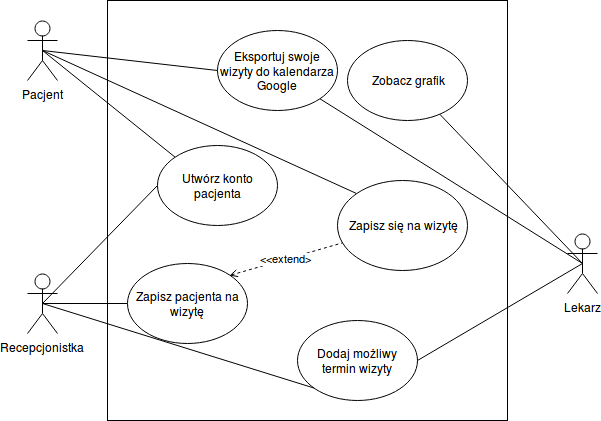
\includegraphics[width=\textwidth]{use-case-v1}
        \caption{\emph{Diagram przypadków użycia} systemu rejestracji pacjentów.}
        \label{use-case-v1}
\end{figure}

Opis przypadków użycia z rys. \ref{use-case-v1}:
\begin{itemize}
    \item 
        \begin{itemize}
            \item Tytuł: Zapisz się na wizytę;
            \item Główny aktor: Pacjent;
            \item Zakres: Systemowy;
            \item Poziom: Cel użytkownika;
        \end{itemize}
\item 
        \begin{itemize}
            \item Tytuł: Odwołaj swoją wizytę;
            \item Główny aktor: Pacjent;
            \item Zakres: Systemowy;
            \item Poziom: Cel użytkownika;
        \end{itemize}
\item 
        \begin{itemize}
            \item Tytuł: Utwórz konto pacjenta;
            \item Główny aktor: Pacjent lub Recepcjonistka;
            \item Zakres: Systemowy;
            \item Poziom: Cel użytkonika;
        \end{itemize}
\item 
        \begin{itemize}
            \item Tytuł: Eksportuj swoje wizyty do kalendarza Google;
            \item Główny aktor: Pacjent lub Lekarz;
            \item Zakres: Organizacji;
            \item Poziom: Podfunkcja;
        \end{itemize}
\item 
        \begin{itemize}
            \item Tytuł: Zobacz grafik;
            \item Główny aktor: Lekarz;
            \item Zakres: Organizacji;
            \item Poziom: Cel użytkownika;
        \end{itemize}
\item 
        \begin{itemize}
            \item Tytuł: Przeglądaj terminy i wizyty w kalendarzu;
            \item Główny aktor: Pacjent, Recepjonistka lub Lekarz;
            \item Zakres: Podfunkcja;
            \item Poziom: Systemowy;
        \end{itemize}
\item 
        \begin{itemize}
            \item Tytuł: Usuń termin wizyty
            \item Główny aktor: Pacjent lub Recepcjonistka,
            \item Zakres: Cel użytkownika;
            \item Poziom: Systemowy;
        \end{itemize}
\item 
        \begin{itemize}
            \item Tytuł: Odwołaj wizytę;
            \item Główny aktor: Recepcjonistka lub Lekarz;
            \item Zakres: Cel użytkownika;
            \item Poziom: Systemowy;
        \end{itemize}
\item 
        \begin{itemize}
            \item Tytuł: Zapisz pacjenta na wizytę;
            \item Główny aktor: Recepcjonistka;
            \item Zakres:;
            \item Poziom:;
        \end{itemize}
\item 
        \begin{itemize}
            \item Tytuł: Dodaj termin wizyty;
            \item Główny aktor: Recepcjonistka lub Lekarz;
            \item Zakres: Cel użytkownika;
            \item Poziom: Systemowy;
        \end{itemize}
\end{itemize}
 
\subsubsection{Wymagania niefunkcjonalne}
Wymagania pozafunkcjonalne specyfikują kryteria osądzania działania systemu. Są one znane jako wymagania jakościowe.
\begin{itemize}
    \item Aplikacja ma wykorzystywać \href{https://getbootstrap.com/}{Twitter Bootstrap} do stworzenia interfejsu użytkownika --- jest to ustalone ze względu na wymaganie zachowania spójności wyglądu z produktami zależnymi.
    \item W warstwie bazodanowej ma być używana relacyjna baza danych --- jest to ustalone ze względu na kompatybilność z produktami zależnymi.
    \item Aplikacja ma działać w przeglądarce internetowej.
    \item Aplikacja ma działać na komputerach stacjonarnych, laptopach oraz tabletach.
    \item Aplikacja ma działać dla wielu współbieżnych użytkowników.
    \item Aplikacja ma być łatwa w obsłudze dla personelu gabinetu lekarskiego oraz pacjentów.
\end{itemize}


\section{Wybrane aspekty realizacji}
%\section{Selected realization aspects}
\label{sec:wybrane-aspekty-realizacji}

Poniżej opisano dziedzinę, strukturę i zasadę działania systemu.

\subsection{Analiza technologiczna}
\label{subsec:analizaTechnologiczna}
Analiza odbywa się według warstw logicznych aplikacji, które zostaną bardziej szczegółowo omówione przy opisie architektury systemu.

\subsubsection{Aplikacja przeglądarkowa}
Wykorzystane technologie:
\begin{itemize}
  \item \href{https://pl.wikipedia.org/wiki/HTML}{HTML},
  \item \href{https://pl.wikipedia.org/wiki/JavaScript}{JavaScript},
  \item \href{https://jwt.io/}{JWT} - dla bezpieczeństwa komunikacji i utrzymania sesji użytkownika.
\end{itemize}

Dla polepszenia satysfakcji klienta i uspójnienia wyglądu z innymi modułami wykorzystamy zręby
\begin{itemize}
  \item \href{https://getbootstrap.com/}{Twitter Bootstrap}.
\end{itemize}

\subsubsection{Warstwa logiki biznesowej}
Będzie to serwer HTTP API, komunikaty będziemy przesyłać w standardzie JSON \\
Wykorzystane technologie:
\begin{itemize}
  \item \href{https://pl.wikipedia.org/wiki/Hypertext_Transfer_Protocol}{HTTP} - zwłaszcza metody \emph{GET} i \emph{POST},
  \item \href{http://www.json.org/}{JSON},
  \item \href{https://www.oracle.com/java/index.html}{Java}.
\end{itemize}

\subsubsection{Baza danych}
\label{subsec:wykorzystane-technologie-baza}
Wykorzystamy relacyjną bazę danych --- dane pacjentów i rejestracji są relacyjne. Problemem tego podejścia jest mała elastyczność. \\
Elastyczność jest wymagana ze względu na potrzebę wspierania różnych formularzy dla pacjentów w zależności od typu gabinetu lekarskiego oraz różnych formularzy dla pacjentów w zależności od potrzeb lekarza. \\
Ten problem rozwiążemy przechowując pliki \emph{JSON}-owe w bazie danych. Jest to rozwiązanie mało eleganckie lecz usprawiedliwione prostotą implementacji. Stworzenie i poprawna implementacja relacyjnego modelu danych posiadającego wymaganą elastyczność wymagało by więcej czasu niż jesteśmy w stanie poświęcić pracy inżynierskiej. \\
Wykorzystane technologie:
\begin{itemize}
  \item \href{https://www.postgresql.org/}{PostgreSQL}.
\end{itemize}


\subsection{Dziedzina problemu}

Zadane środowisko w którym jest osadzony produkt.

\subsubsection{Przeglądarka internetowa}
Użytkownik komunikuje się z aplikacją za pośrednictwem przeglądarki internetowej. Przeglądarka to program komputerowy służący do pobierania i wyświetlania stron internetowych udostępnianych przez serwery WWW (rys. \ref{html-css-js} i \ref{http_diagram}).

\begin{figure}[H]
    \centering
    \begin{minipage}{0.45\textwidth}
        \centering
        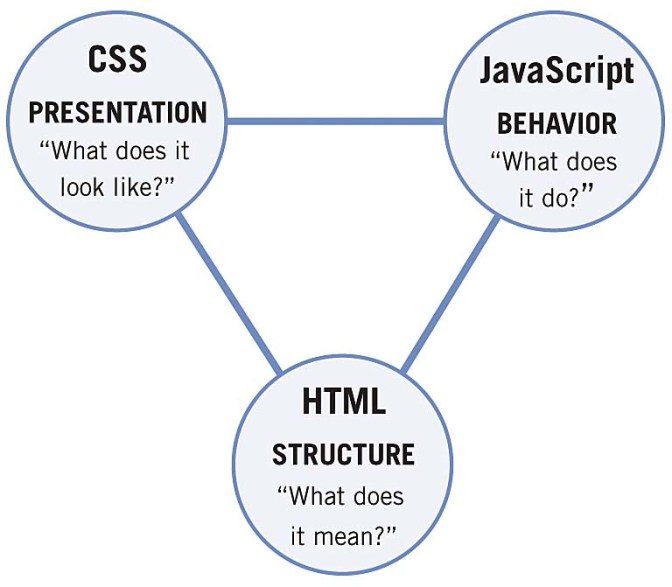
\includegraphics[width=0.9\textwidth]{html-css-js} % first figure itself
        \caption{Strony internetowe są tworzone z użyciem HTML-a, CSS-a i JavaScript-a}
        \label{html-css-js}
    \end{minipage}\hfill
    \begin{minipage}{0.45\textwidth}
        \centering
        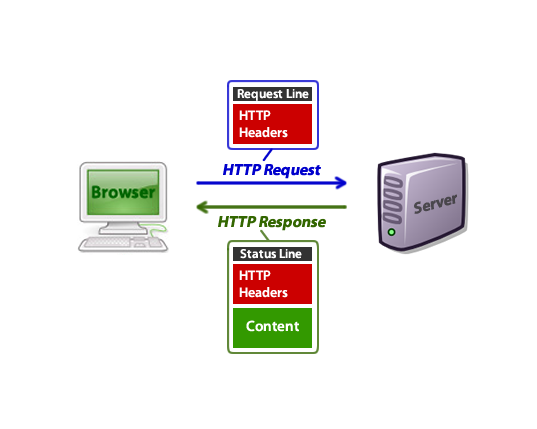
\includegraphics[width=0.9\textwidth]{http_diagram} % second figure itself
        \caption{Przeglądarka internetowa pobiera strony internetowe używając protokołu HTTP}
        \label{http_diagram}
    \end{minipage}
\end{figure}


\subsection{Wstęp - zarys architektury systemu}
Produkt posiada architekturę trójwarstwową. Składają się na nią:
\begin{itemize}
    \item Aplikacja przeglądarkowa (warstwa prezentacji) --- udostępnia interfejs użytkownika, tworzy zapytania do warstwy logiki biznesowej, wysyła do niej dane i prezentuje otrzymane zeń wyniki,
    \item Warstwa logiki biznesowej --- udostępnia właściwą (biznesową) funkcjonalność systemu, obsługując zapytania klienta (w tym wypadku aplikacji wykonującej się w przeglądarce); przetwarza dane klienta, a także wykonuje operacje na bazie danych,
    \item Warstwa bazodanowa --- odpowiada za przechowywanie danych i udostępnia funkcjonalność ich zapisu i odczytu.
\end{itemize}

Na rysunku \ref{architektura} przedstawiona jest ogólna architektura całego systemu na wysokim poziomie abstrakcji.

\begin{figure}[H]
    \centering
    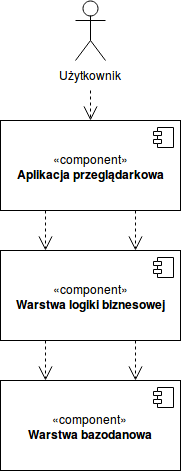
\includegraphics{architektura}
    \caption{Architektura systemu na wysokim poziomie abstrakcji}
    \label{architektura}
\end{figure}


\subsection{Aplikacja przeglądarkowa}
Aplikacja przeglądarkowa udostępnia interfejs użytkownika i komunikuje się z warstwą logiki biznesowej. Aplikacja wykonuje się w przeglądarce internetowej na urządzeniu użytkownika.

\subsubsection{Zarys architektury}
Poniżej przedstawiamy poglądowy schemat architektury aplikacji przeglądarkowej (rys. \ref{front-schema}) i opis poszczególnych komponentów.

\begin{figure}[H]
    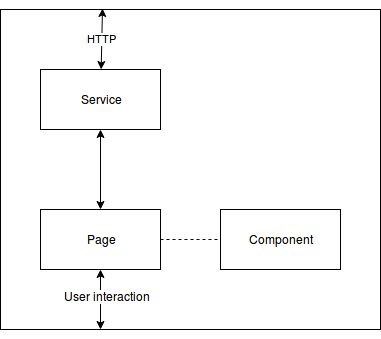
\includegraphics[width=\textwidth]{front-schema}
    \caption{Poglądowy schemat architektury aplikacji przeglądarkowej}
    \label{front-schema}
\end{figure}

Komponenty aplikacji przeglądarkowej:
\begin{itemize}
    \item Service - serwisy odpowiadają za wysyłanie zapytań do aplikacji serwerowej i odbieranie odpowiedzi.
    \item Page - Trasowalna strona wyświetlana użytkownikowi.
    \item Component - Strony korzystają z komponentów.
\end{itemize}

\subsubsection{Technologie}
Technologie informatyczne wykorzystane przy tworzeniu produktu.
\paragraph{Angular 2} - zręby aplikacji przeglądarkowej. Umożliwiają:
\begin{itemize}
    \item wysyłanie i odbieranie zapytań HTTP,
    \item dynamiczną zmianę zawartości strony internetowej.
\end{itemize}
\subsubsection{Serwisy}
Serwisy służą do wysyłania zapytań HTTP. Ich metody zwracają \emph{Promise}. Serwisy służące rejestracji pacjentów:
\begin{itemize}
    \item authentication service,
    \item appointment service,
    \item doctor service,
    \item google calendar service,
    \item patient service,
    \item timeSlot service,
    \item user service.
\end{itemize}
\paragraph{Zależności między serwisami} ---
 graf pokazuje, których serwisów trzeba użyć aby uzyskać całość danych na temat danej encji. \\
 Na przykład aby uzyskać całość danych na temat \emph{Appointment} trzeba znać \emph{TimeSlot}, \emph{Doctor}-a przyjmującego wizytę i \emph{Patient}-a zapisanego na wizytę.
 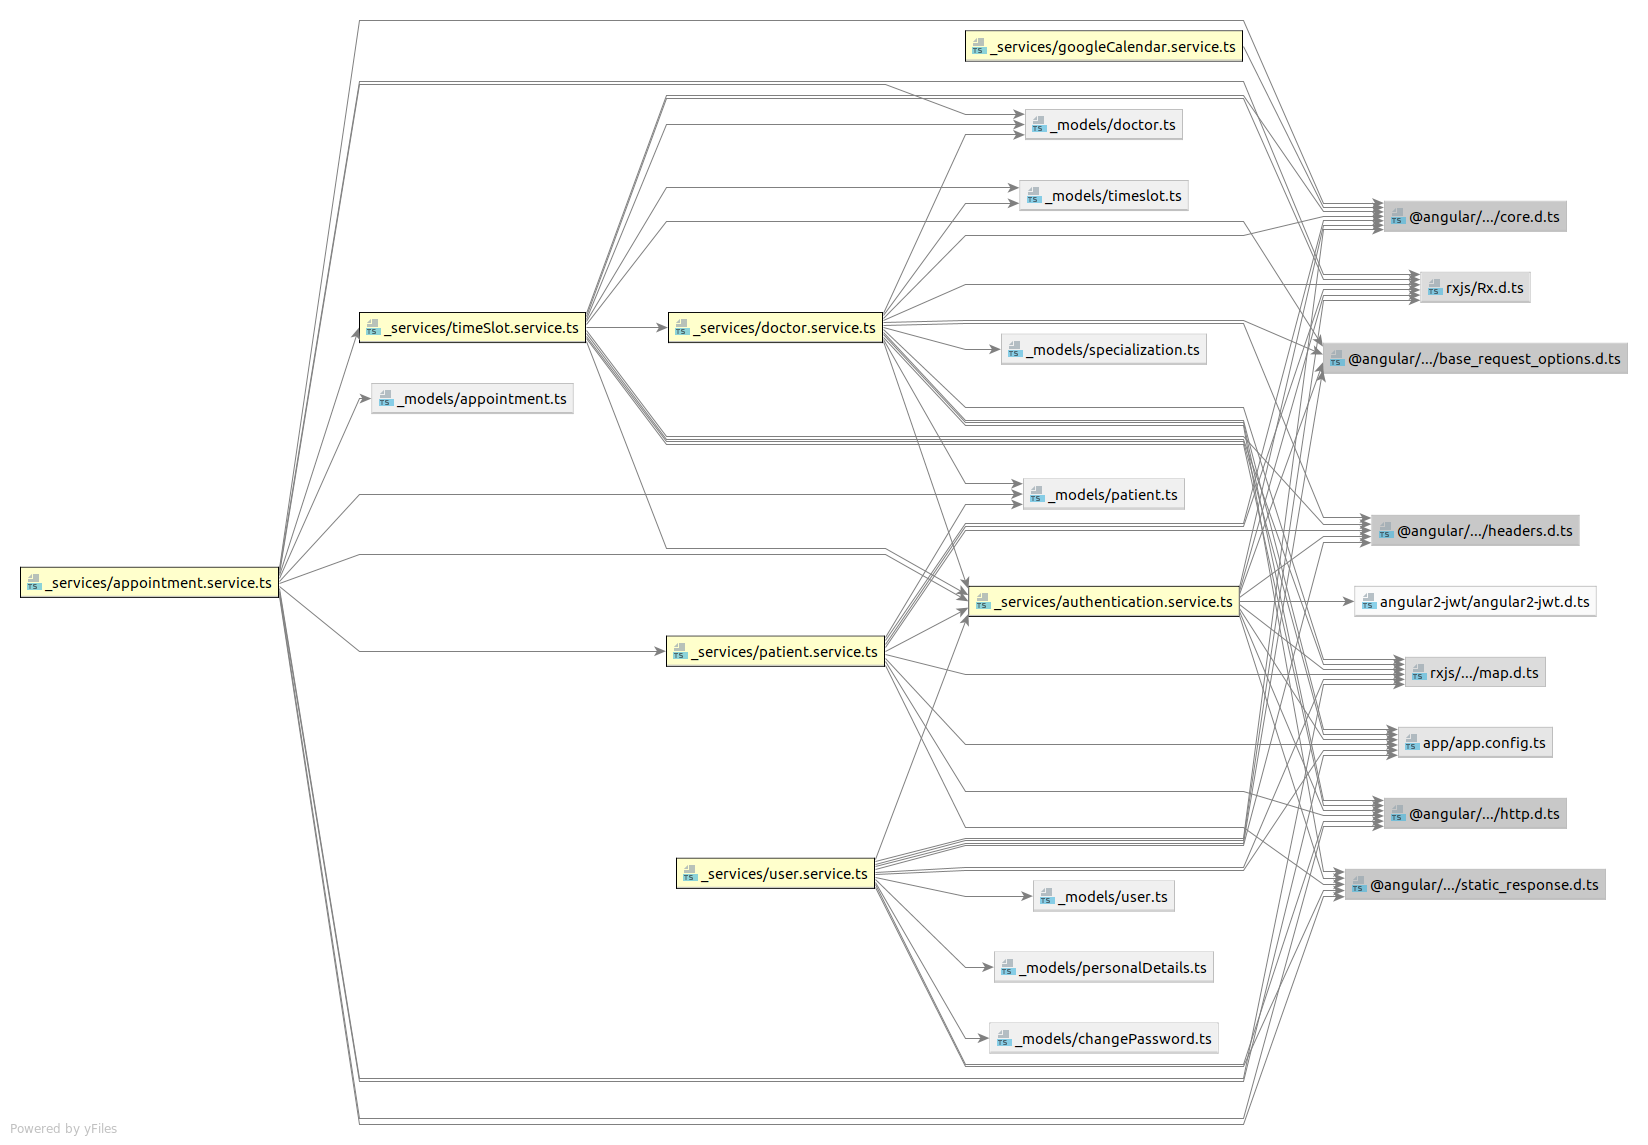
\includegraphics[width=\textwidth]{services-dep}

\subsubsection{Kalendarz terminów}
Kalendarz jest kluczowym elementem interfejsu systemu rejestracji.
\paragraph{Diagram zależności} pokazuje wszystkie zależności komponentu kalendarza.
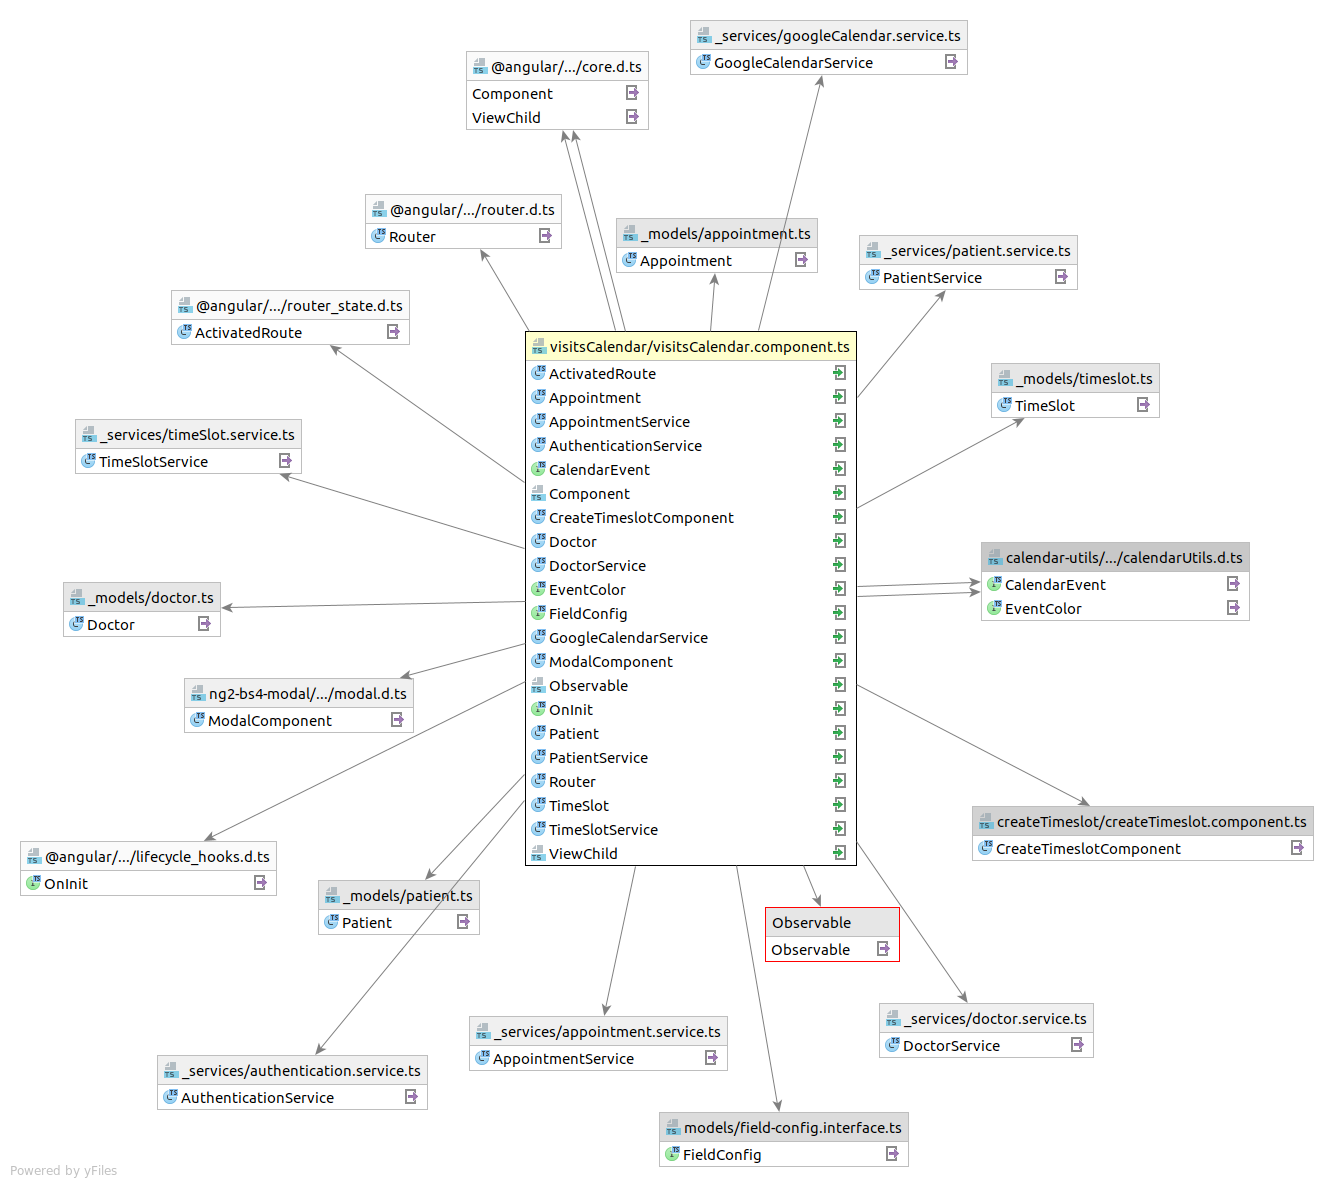
\includegraphics[width=\textwidth]{visitsCalendar_dep}
\paragraph{Inicjalizacja kalendarza} ---
inicjalizacja wygląda inaczej w zależności od tego, kto otwiera widok kalendarza.
\begin{itemize}
    \item Pacjent \\
     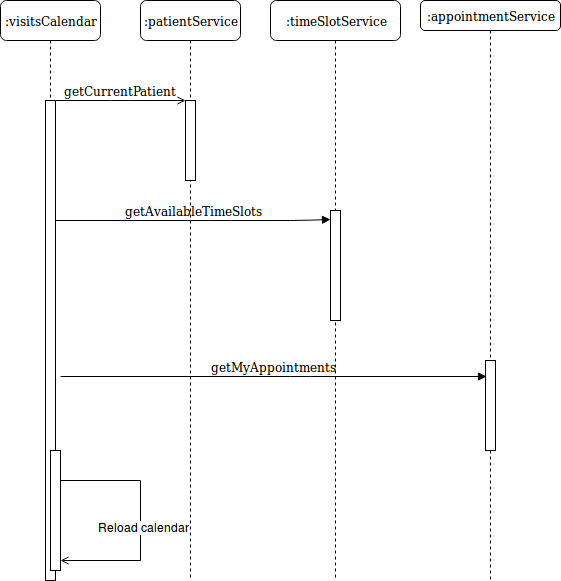
\includegraphics[width=\textwidth]{patient-init-cal},
    \item Doktor \\
    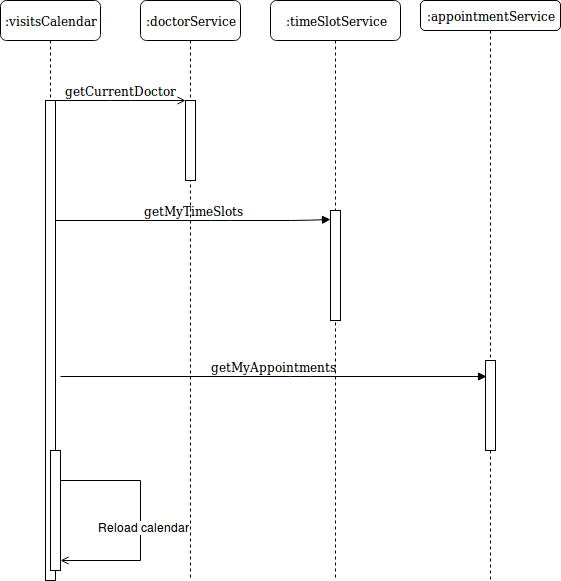
\includegraphics[width=\textwidth]{doctor-init-cal},
    \item Recepcjonistka \\
    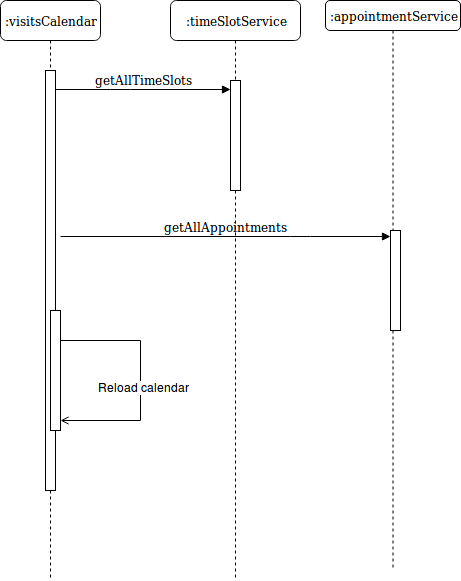
\includegraphics[width=\textwidth]{cal-recep-init}.
\end{itemize}

%\paragraph{Zapis i modyfikacja danych}


\paragraph{Eksport terminów z kalendarza do 'Google Calendar' \footnote{Specyfikacja API znajduje się \href{https://www.googleapis.com/discovery/v1/apis/calendar/v3/rest}{tutaj}}} odbywa się wg schematu
\begin{enumerate}
    \item Zaloguj się - użytkownik zostaje przekierowany na stronę, logowania Google, po zalogowaniu aplikacja otrzymuje jego token oAuth
    \item Dodaj wydarzenie do kalendarza,
    \item Wyloguj się - token jest unieważniany.
\end{enumerate}


\subsubsection{Formularze}
Formularze do tworzenia pacjentów, doktorów, terminów wizyt itp. są oparte o komponent \emph{DynamicForm} autorstwa powiązanego zespołu \emph{Health Manager}.
Ich konfiguracją jest lista JSON-owa. Przykład dla tworzenia dostępnych terminów (\emph{createTimeslot.component.ts})
\begin{verbatim}
    [
        {
            type: 'select',
            label: 'Doctor',
            name: 'doctor',
            placeholder: 'Select a doctor',
            options: []
        },
        {
            type: 'date',
            label: 'Start Date-time',
            name: 'startDateTime'
        },
        {
            type: 'date',
            label: 'End Date-time',
            name: 'endDateTime'
        },
        {
            type: 'checkbox',
            label: 'Available for self-sign',
            name: 'availableForSelfSign',
            value: true
        },
        {
            label: 'Submit',
            name: 'submit',
            type: 'button'
        }
    ];
\end{verbatim}
Każdy obiekt na liście konfigurującej odpowiada jednemu komponentowi do wprowadzania danych. Obiekty listy konfiguracji muszą mieć pola:
\begin{itemize}
    \item \texttt{type} --- typ komponentu, może przyjmować wartości: 'select', 'date', 'checkbox', 'input', 'button';
    \item \texttt{label} --- nazwa widocza dla użytkownika, dowolny ciąg znaków;
    \item \texttt{name} --- nazwa która będzie identyfikowała komponent w kodzie, niewidoczna dla użytkownika;
    \item \texttt{value} [opcjonalne] --- domyślna wartość dla komponentu. Dostępne wartości zależą od rodzaju komponentu.
\end{itemize}


\subsection{Warstwa logiki biznesowej}
Warstwa logiki biznesowej udostępnia właściwą funkcjonalność systemu jako \emph{usługę sieciową} (ang. \emph{web service}) zaprojektowaną wg zasad \emph{REST}\footnote{z ang. \emph{Representational State Transfer}} na protokole HTTP.

\subsubsection{Zarys architektury}
Poniżej przedstawiamy poglądowy schemat architektury warstwy logiki biznesowej (rys. \ref{backedn-schema}) i opis poszczególnych komponentów.

\begin{figure}[H]
    \centering 
    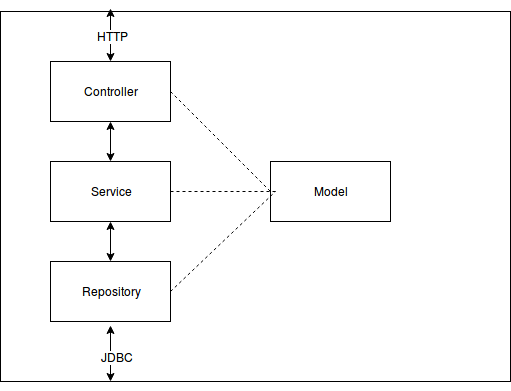
\includegraphics[width=\textwidth]{backedn-schema}
    \caption{Poglądowy schemat architektury warstwy logiki biznesowej}
    \label{backedn-schema}
\end{figure}

Komponenty warstwy logiki biznesowej:
\begin{itemize}
    \item Controller - warstwa odpowiedzialna za odbieranie zapytań HTTP i przetwarzanie ich na obiekty JVM-owe oraz za przetwarzanie odpowiedzi (obiektów JVM-owych) na wiadomości HTTP i odsyłanie ich.
    \item Service - warstwa pośrednicząca międzu Controller-em a Repository-em. Przetwarza zapytania otrzymane od Controllera na zapytania dla Repository i przetwarza odpowiedzi od Repository na odpowiedzi dla Controller-a.
    \item Repository - warstwa odpowiedzialna za wykonywanie zapytań do bazy danych.
    \item Model - wspóny dla wyżej wymienionych warstw sposób reprezentacji encji jako obiektów JVM-kowych, który może być przetworzony na JSON-a (na potrzeby HTTP API) lub repotezentację bazodanową (na potrzeby bazy danych). Umożliwia komunikację pomiędzy Controller-em, Servic-em i Repository-em.
\end{itemize}
\subsubsection{Technologie}
Wykorzystano język programowania Java oraz biblioteki Spring i Hibernate.
\paragraph{Spring} pozwala na:
\begin{itemize}
    \item odbieranie i wysyłanie zapytań HTTP,
    \item używanie CRUD-owego API do bazy danych.
\end{itemize}
\paragraph{Hibernate} pozwala na:
\begin{itemize}
    \item utworzenie schematu bazy danych na podstawie klas Javy,
    \item serializację i zapis obiektów Javy,
    \item odczyt z bazy obiektów Javy.
\end{itemize}
\subsubsection{Modelowane encje}
Poniżej znajduje się spis (w formie obrazków) encji modelowanych na potrzeby produktu.
    \paragraph{Timeslot} - możliwy termin wizyty u danego lekarza.
    \begin{figure}[H]
    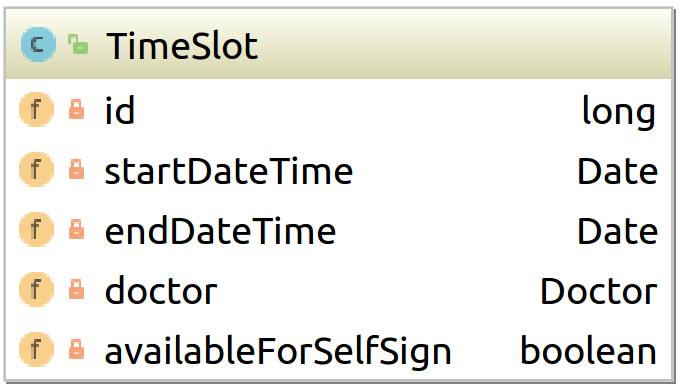
\includegraphics[width=0.7\textwidth]{TimeSlot}
    \caption{Nie zawiera informacji czy termin jest zarezerwowany, może być interpretowany jako czas w którym lekarz na pewno jest w pracy}
    \end{figure}
    \paragraph{Appointment} - Zarezerwowany termin u wizyty
    \begin{figure}[H]
    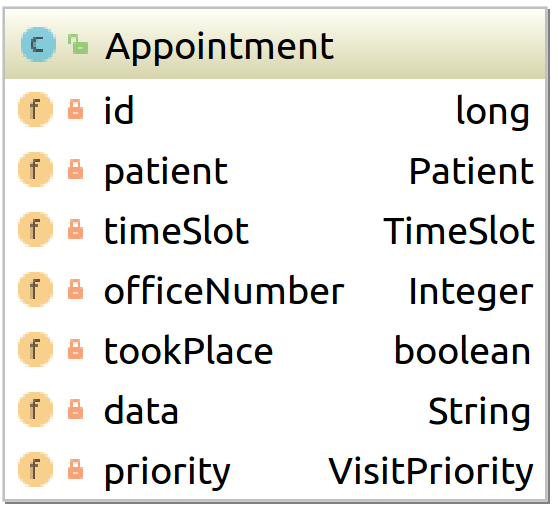
\includegraphics[width=0.7\textwidth]{Appointment}
    \caption{Zawiera szczegóły rezerwacji, jak na przykład dane pacjenta czy priorytet wizyty.
    Zawiera w sobie \emph{TimeSlot} - czyli informację o terminie i lekarzu przyjmującym wizytę}
    \end{figure}
    \paragraph{Doctor} - lekarz 
    \begin{figure}[H] 
    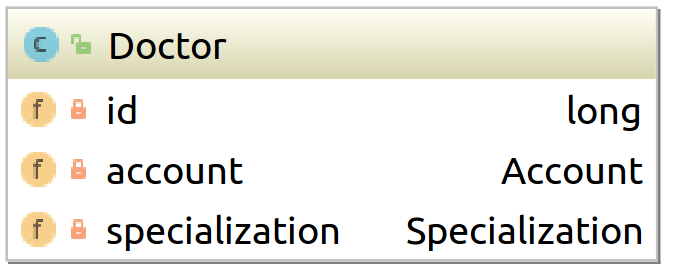
\includegraphics[width=0.7\textwidth]{Doctor} 
    \caption{Encja lekarza odpowiada jednej jego specjalizacji}
    \end{figure}
    \paragraph{Patient} - pacjent 
    \begin{figure}[H]
    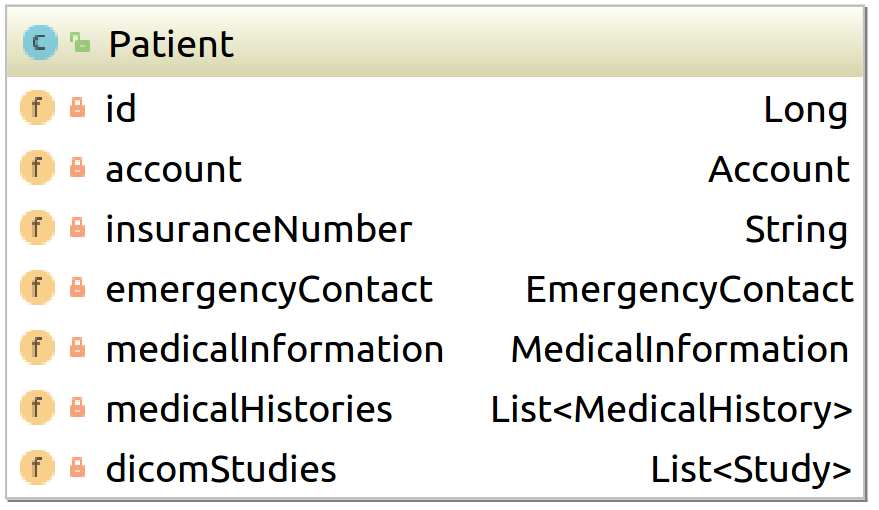
\includegraphics[width=0.7\textwidth]{Patient}
    \end{figure}
    \paragraph{Account} - konto w systemie 
    \begin{figure}[H]
    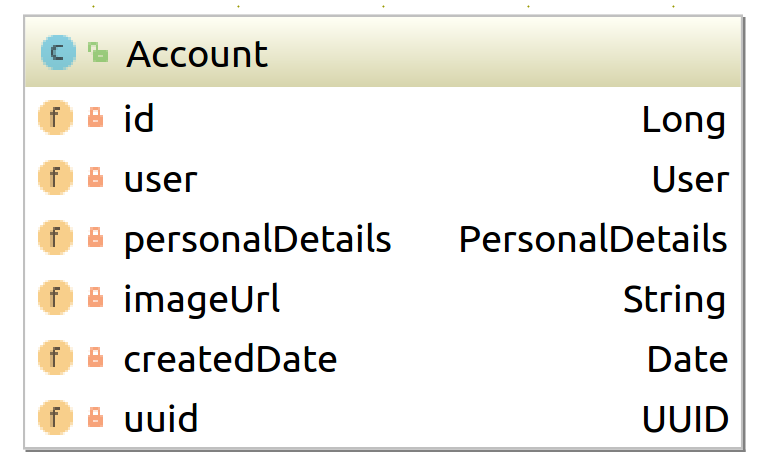
\includegraphics[width=0.7\textwidth]{Account}
    \caption{Konto nie opisuje uprawnień ani hasła użytkownika, jest tylko łącznikiem dla encji \\
    Account zawiera \emph{User} które ma hasło i e-mail użytkownika.}
    \end{figure}
    \paragraph{PersonalDetails} - dane osobowe 
    \begin{figure}[H]
        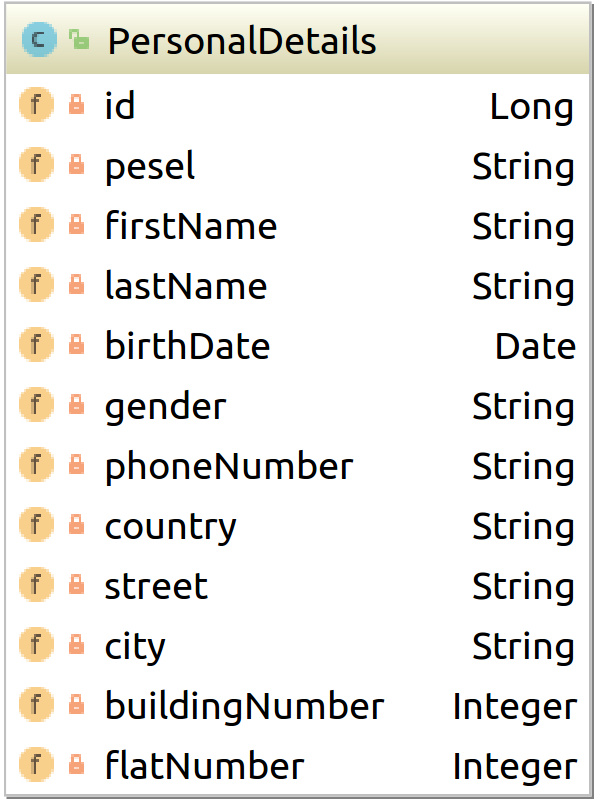
\includegraphics[width=0.7\textwidth]{PersonalDetails}
        \caption{Ta encja dotyczy zarówno lekarza i pacjenta}
    \end{figure}
    \paragraph{User} - dane użytkownika 
    \begin{figure}[H]
    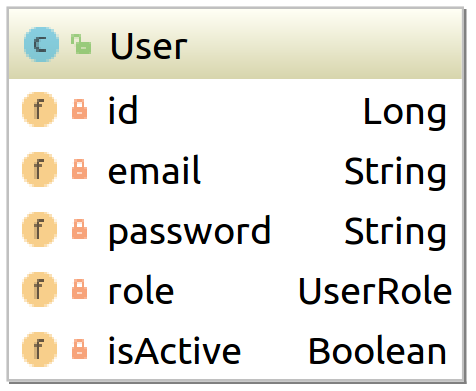
\includegraphics[width=0.7\textwidth]{User}
    \caption{powiązane z \emph{Account}}
    \end{figure}
    \paragraph{Specialization} - specjalizacja lekarza 
    \begin{figure}[H]
    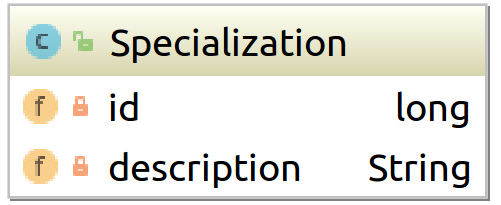
\includegraphics[width=0.7\textwidth]{Specialization}
    \end{figure}
\subsubsection{Powiązanie modelowanych encji}
Powiązanie modelowanych encji odpowiada schematowi relacyjnej bazy danych.
\paragraph{Wersja zwinięta} - Schemat bez widocznych pól
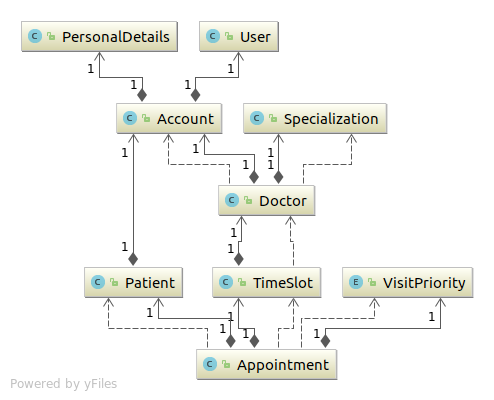
\includegraphics[width=\textwidth]{java-entities-small}
\paragraph{Wersja rozwinięta} - Schemat z widocznymi polami \\
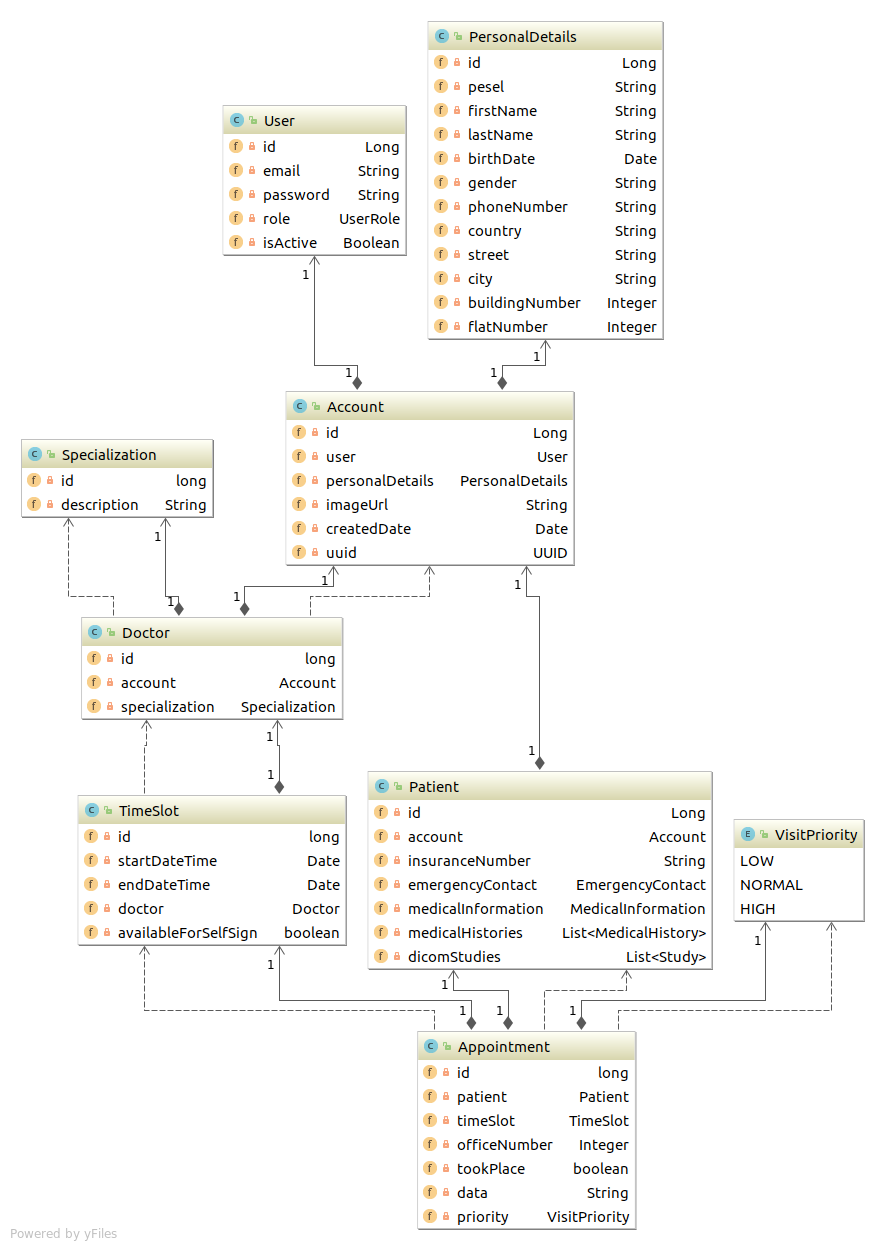
\includegraphics[width=\textwidth]{java-entities-big}

\subsubsection{Obsługa zapytań}
Obsługa wiadomości przychodzących do serwera.
\paragraph{Schemat} --- 
obsługa zapytań HTTP przychodzących do serwera logiki biznesowej ma w większości przypadków następujący przebieg (opisany we wstępie):
\begin{enumerate}
  \item \emph{Kontroler} odbiera zapytanie HTTP i przekazuje serwisowi,
  \item \emph{Serwis} sprawdza poprawność zapytania i wykonuje pod-zapytania do repozytorium,
  \item \emph{Repozytorium} pobiera potrzebne dane z bazy danych i zwraca serwisowi,
  \item \emph{Serwis} przekształca dane otrzymane od repozytorium w odpowiedź na zapytanie i przekazuje odpowiedź kontrolerowi,
  \item \emph{Kontroler} odsyła odpowiedź po HTTP.
\end{enumerate}

\paragraph{Przykład - getTimeSlotById} - zapytanie o dane \emph{TimeSlot}-u na podstawie jego \emph{ID}
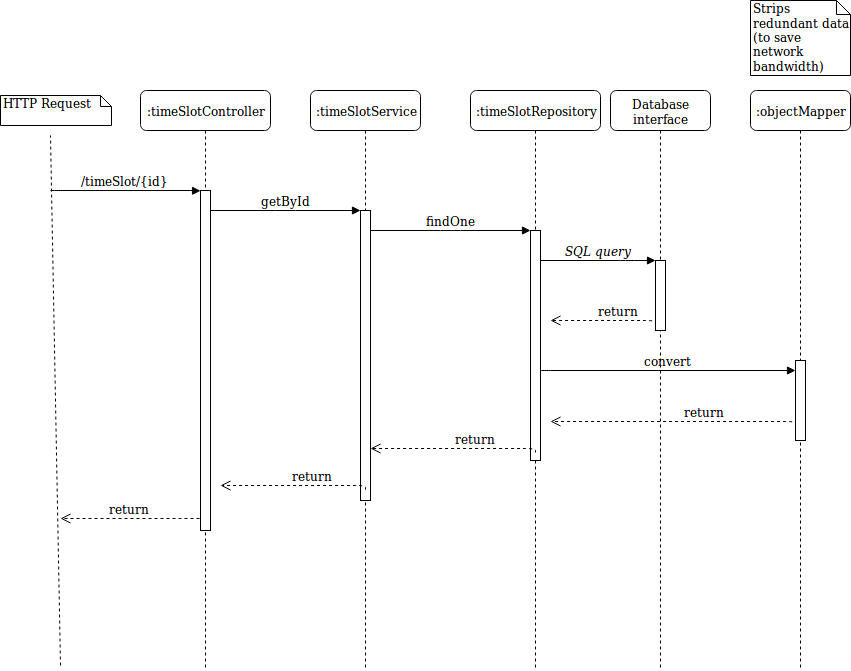
\includegraphics[width=\textwidth]{timeSlotById}

\paragraph{Przykład - getInIntervalForDoctor} --- zapytanie o listę \emph{TimeSlot}-ów dla danego doktora w zadanym przedziale czasowym. \\
Schemat opisany powyżej jest na tyle ogólny że równie dobrze modeluje prostsze zapytanie \emph{getTimeSlotById} jak i bardziej skomplikowane \emph{getInIntervalForDoctor}. Różnica w implementacji występuje na poziomie \emph{repozytorium}, które musi wykonać odpowiednio inne zapytania do bazy danych i \emph{serwisu} który inaczej sprawdza poprawność danych
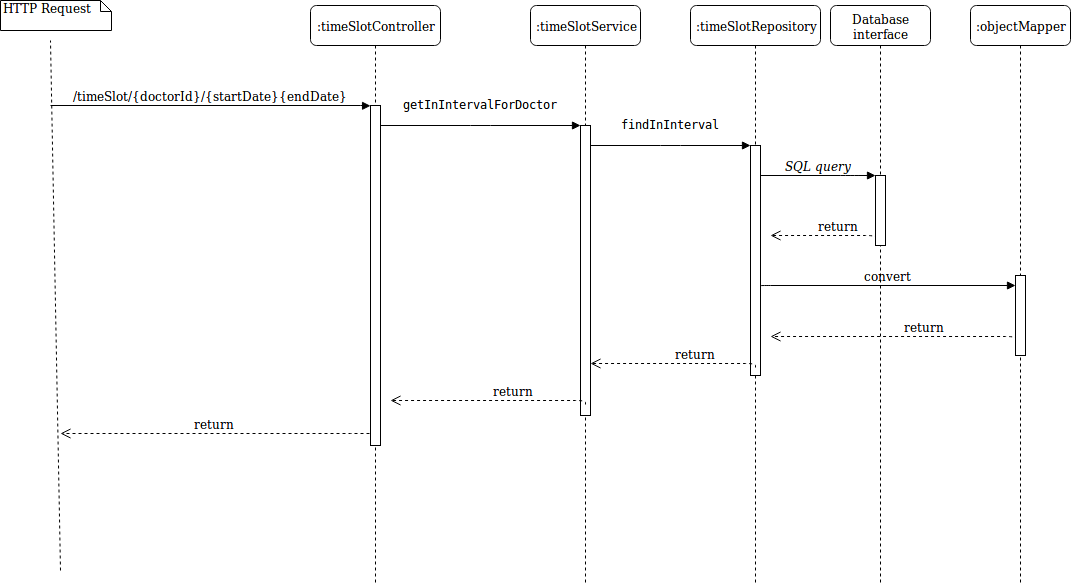
\includegraphics[width=\textwidth]{inIntervalDorDoctor}


\subsection{Baza danych}
Warstwa bazodanowa odpowiada za persystencję danych. Wykorzystano relacyjną bazę danych \emph{PostgreSQL}.

Poniżej przedstawiamy schemat bazy danych (rys. \ref{db-schema}).

\begin{figure}[H]
    \caption{Schemat bazy danych jest tworzony ad-hoc przy starcie aplikacji przez \emph{Hibernate}-a}
    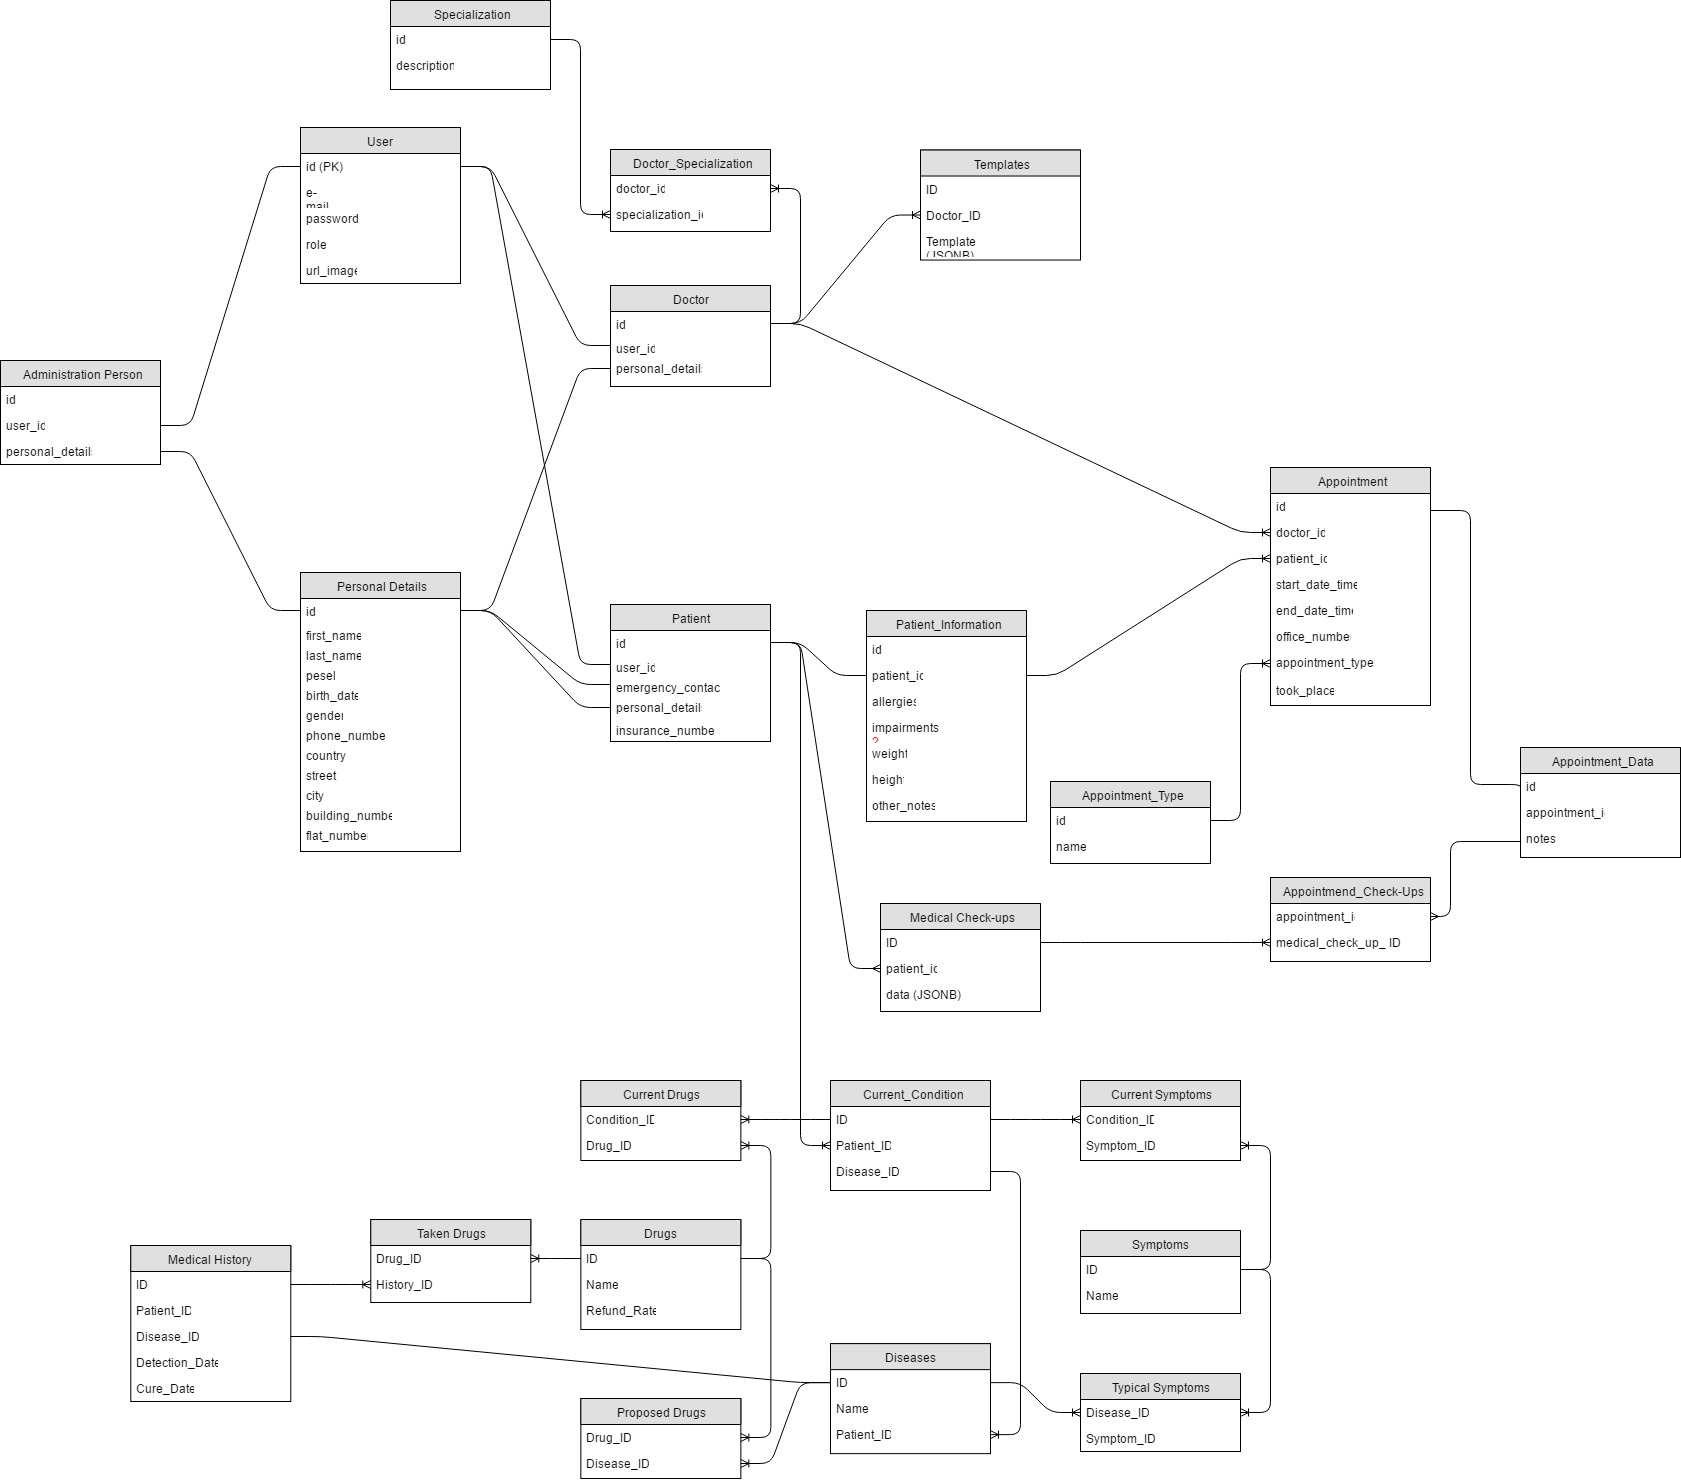
\includegraphics[width=\textwidth]{db-schema}
    \label{db-schema}
\end{figure}


\subsection{Komunikacja aplikacji przeglądarkowej i warstwy logiki biznesowej}
Warstwa logiki biznesowej wystawia API, które zostało zaprojektowane w oparciu o zasady \emph{REST} (ang. \emph{Representational State Transfer}). Aplikacja przeglądarkowa i serwer logiki biznesowej komunikują się przez protokół HTTP, wymieniając pliki JSON.

Przykład komunikacji:

\begin{enumerate}
  \item Lekarz, korzystając z aplikacji klienckiej, wysyła zapytanie o umówiony termin wizyty będące zapytaniem HTTP GET na adres server-addr:8080/appointments/123. "123" to numer identyfikacyjny umówionej wizyty,
  \item Serwer zwraca odpowiedź:
\begin{verbatim}
{    
  id: 123,
  patientId: 32,
  timeSlotId: 432,
  tookPlace: false,
  officeNumber: 10,
  data: "Podejrzenie schizofrenii bezobjawowej!",
  priority: LOW
}
\end{verbatim}.
\end{enumerate}

Wykaz formatu zapytań i odpowiedzi znajduje się w załączniku.

\section{Organizacja pracy}
%\section{Work organization}
\label{sec:organizacja-pracy}

Poniżej opisano strukturę zespołu, metodykę pracy w obrębie zespołu i metodykę współpracy z powiązanymi zespołami.
  
\subsection{Struktura zespołu}
Opis organizacji wewnątrz zespołu.
\subsubsection{Hierarchia zarządzania}
W zespole wyróżniony jest przywódca (wyróżnianie innych funkcji wydało nam się zbędne):
\begin{itemize}
    \item Wojciech Karpiel --- szef, odpowiedzialny za komunikację z Klientem i współpracującymi zespołami,
    \item Filip Galas --- członek zespołu,
    \item Michał Hamuda --- członek zespołu.
\end{itemize}

\subsubsection{Podział technologiczny}
Rozważaliśmy wprowadzenie podziału ze względu na kompetencje techniczne, czyli:
\begin{itemize}
    \item osoba zajmująca się warstwą logiki biznesowej,
    \item osoba zajmująca się aplikacją przeglądarkową.
\end{itemize}
Udało się nam zaimplementować niektóre funkcjonalności, działając wg tego schematu, jednak ostatecznie uznaliśmy to za zbyteczne, ponieważ produkt składa się głównie z kodu aplikacji przeglądarkowej i taki podział funkcji spowodowałby nierównomierny rozkład odpowiedzialności. Zamiast tego każdy członek zespołu odpowiadał za stworzenie front-endowej i back-endowej części funkcjonalności, którą wdrażał.

\subsection{Wyznaczanie i rozdział zadań}
Wykorzystywaliśmy system JIRA, udostępniany przez pracownię IISG. Po każdym spotkaniu z Klientem szef zespołu przetwarzał wymagane przez Klienta funkcjonalności na bilety JIRA. Każde zadanie opisywało jedną funkcjonalność. Zadania były posortowane według istotności (to znaczy: funkjonalności, które należało zaimplementować do następnego spotkania z klientem, były umieszczone najwyżej; najniżej były nasze pomysły, których Klient nie wymagał). Członkowie zespołu, według czasu i możliwości, przypisywali sobie zadania i wykonywali je.
 \begin{figure}[H]
    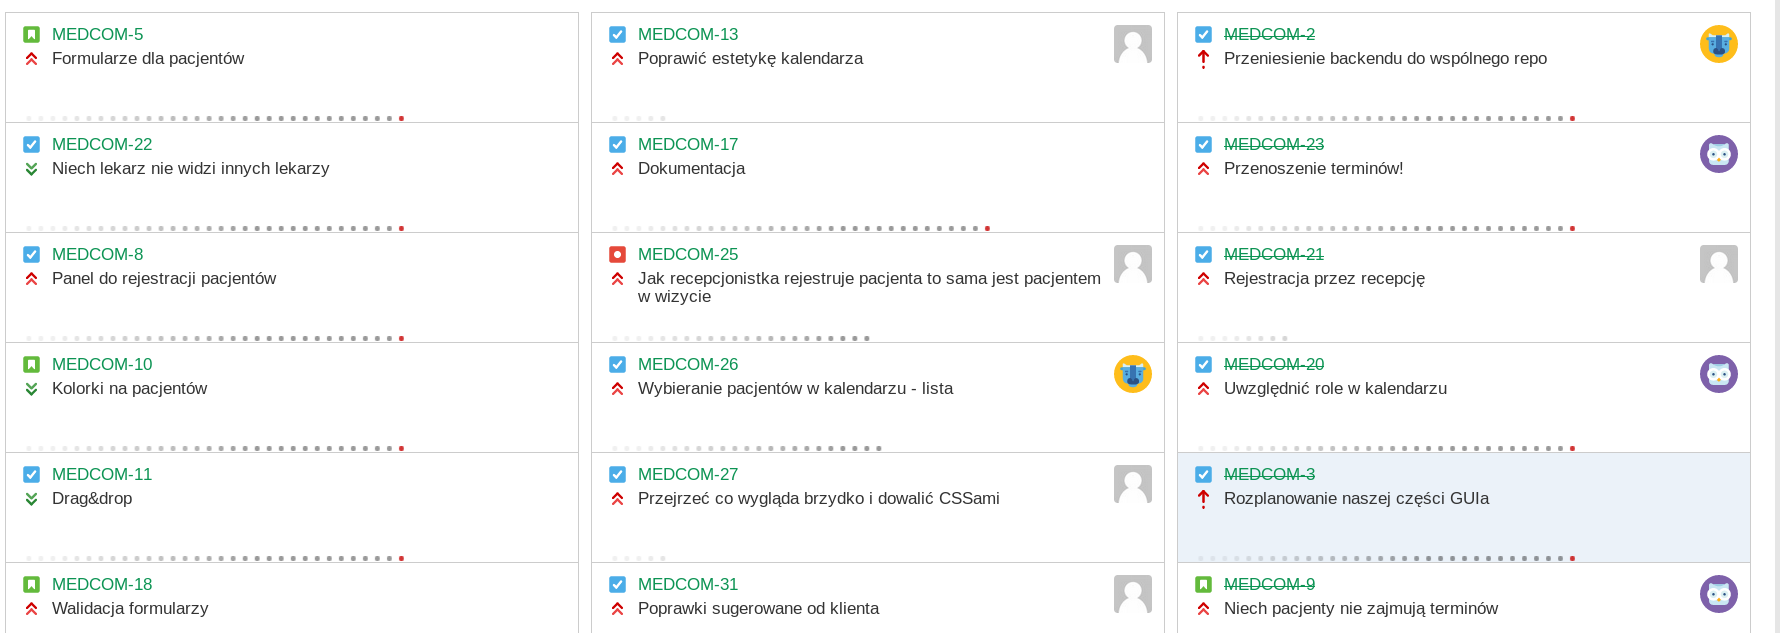
\includegraphics[width=0.7\textwidth]{jira-kanban}
    \caption{Tablica kanbanowa projektu PRZEMEK - element zwinnej metodyki tworzenia oprogramowania}
    \end{figure}

\subsection{Sposób wykonywania zadań}
Produkt składa się de facto z dwóch powiązanych pod-projektów: części front-endowej i back-endowej. Te dwa pod-projekty były objęte systemem kontroli wersji --- Git. Dla każdego pod-projektu osobno członek zespołu tworzył gałąź Gita przypisaną danej funkcjonalności i do niej commitował kod wprowadzający funkcjonalność. Po zakończeniu pracy, pozostali członkowie zespołu przeglądali kod na gałęzi i ewentualnie prosili o wprowadzenie poprawek (code-review). Na końcu gałąź funkcjonalnościowa była dołączana do głównej gałęzi.

\subsection{Komunikacja z powiązanymi zespołami}
Opis organizacji współpracy z powiązanymi zespołami.
\subsubsection{Komunikacja bieżąca}
Do komunikacji bieżącej używaliśmy komunikatora Skype. Według potrzeb, umawialiśmy się na tak zwane call-e, podczas których przedstawiciele każdego z powiązanych zespołów omawiali stan prac i planowali przyszłą pracę.
\subsubsection{Wymiana wiedzy}
Używaliśmy systemu Confluence, udostępnianego przez pracownię IISG. Służył on jako pamięć długotrwała oraz punkt wymiany informacji między zespołami. Tam spisywaliśmy notatki ze spotkań (zarówno tych z Klientem jak i między-zespołowych), prowadziliśmy kalendarz przyszłych spotkań oraz spisywaliśmy różnorakie informacje, które wydawały się nam przydatne. Do Confluence-a mieli dostęp również członkowie powiązanych zespołów.
 \begin{figure}[H]
    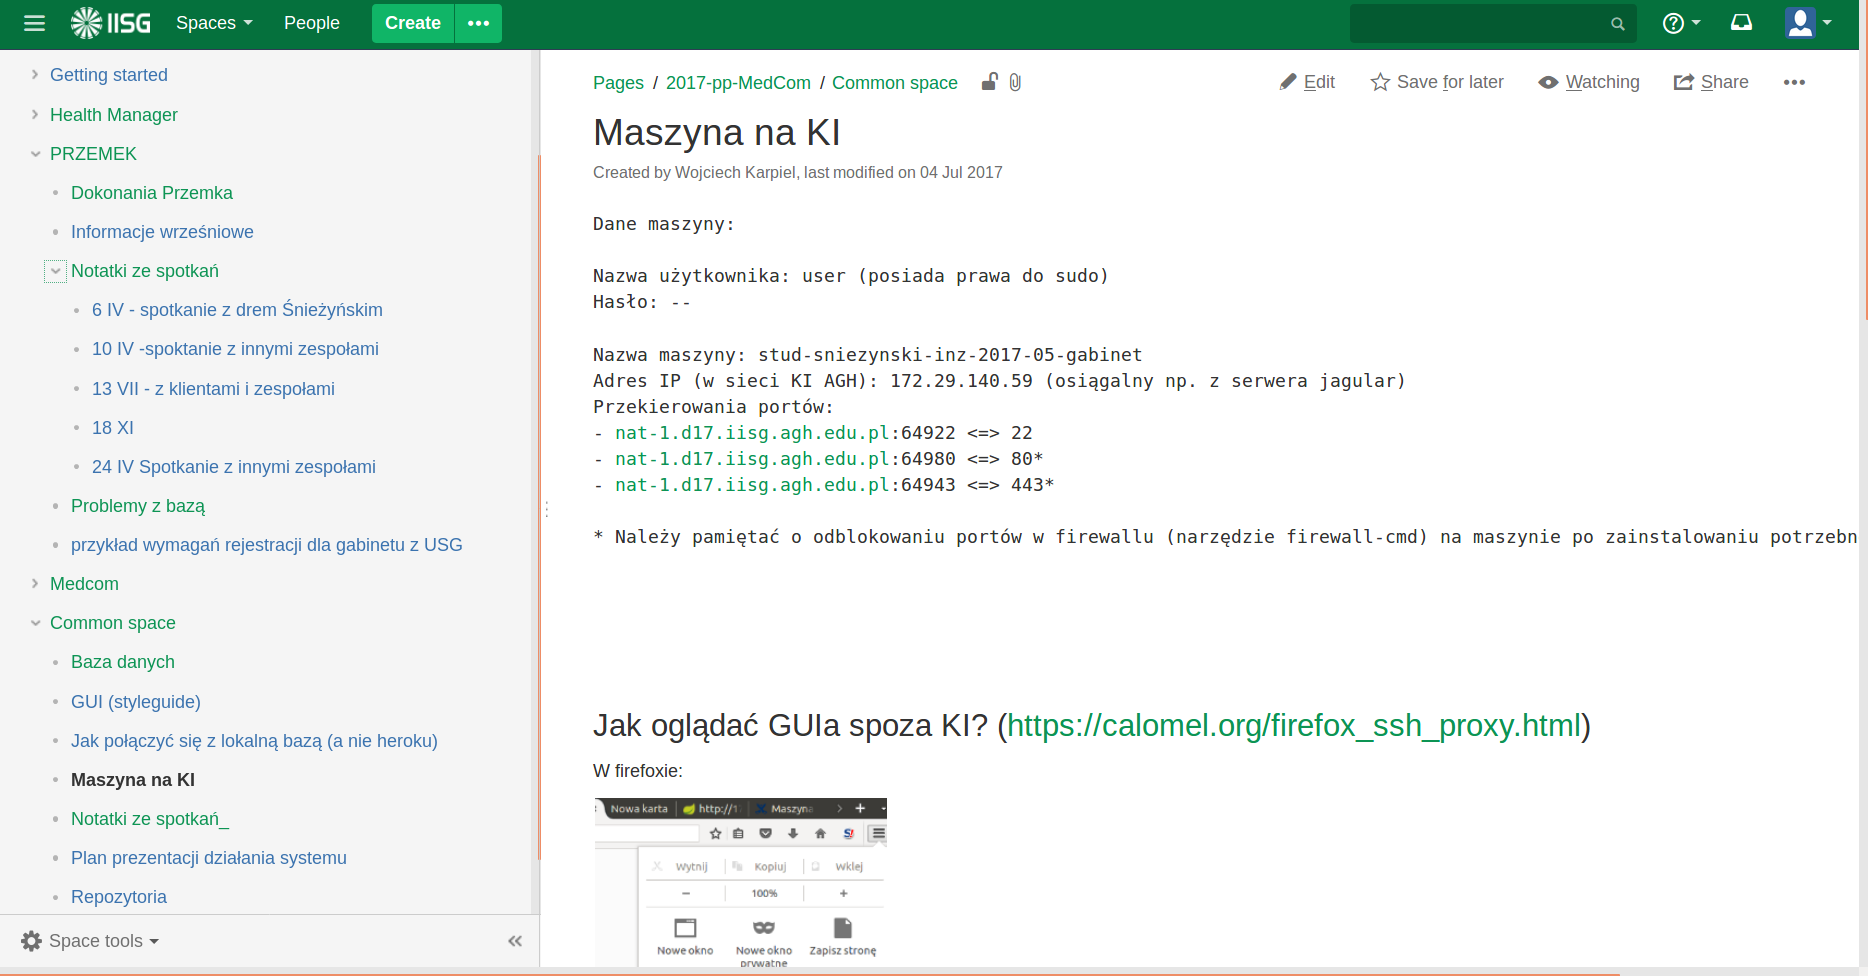
\includegraphics[width=0.7\textwidth]{confluence-maszyna}
    \caption{Strona na Confluence - oprogramowaniu wspomagającym współpracę przy tworzeniu oprogramowania}
    \end{figure}
    
\subsection{Spotkania z Klientem}
Naszym Klientem był dr Bartłomiej Śnieżyński, natomiast Klientem powiązanych zespołów był dr Piotr Nawrocki. Razem z zespołami powiązanymi prosiliśmy naszych Klientów o wspólne spotkania (3 zespoły i 2 Klientów), na co nasi Klienci chętnie przystali. Taka organizacja spotkań ułatwiła koordynację i integrację zespołów.
  
  
\subsection{Podział prac ze względu na osobę wykonującą}
Tabelę utworzono na podstawie Kanbanu produktu.
\begin{center}
  \begin{tabular}{ | l | l | }
    \hline
    %%% TODO
    %%% WSZYSTKO TRZEBA POROZDZIELAĆ NA JAK NAJDROBNIEJSZE SZCZEGÓLIKI
    %%% TAK ŻEBY WYSZŁO ŻE DUŻO ZROBILIŚMY xDD
    %%% TA CZĘŚĆ JEST WAŻNA BO O NIĄ NAWROCKI PROSIŁ 2 RAZY
    %%% można np dopisać kto jakie endpointy dodawał
    Wynik pracy & Osoba wykonująca \\ \hline \hline
    Prototyp  porzucany front-endu\footnote{Nie został w żadnej części wykorzystany we właściwym produkcie ze względu na niezgodność wykorzystanych technologii} & Michał Hamuda \\ \hline
    Projekt HTTP API & Filip Galas \\ \hline
    Prototyp back-endu\footnote{Został częściowo wykorzystany we właściwym produkcie} & Filip Galas  \\ \hline
    Wizja projektu\footnote{Tworzona na potrzeby Pracowni projektowej} & Wojciech Karpiel \\ \hline
    Podział części front-endowej na komponenty & Michał Hamuda \\ \hline
    Osadzenie komponentów części front-endowej w ogólnym szkielecie aplikacji & Michał Hamuda \\ \hline
    Konfiguracja bibliotek używanych w części front-endowej & Michał Hamuda \\ \hline
    Kalendarz lekarza & Michał Hamuda \\ \hline
     Kalendarz pacjenta & Michał Hamuda \\ \hline
    Możliwość przenoszenia terminów & Wojciech Karpiel \\ \hline
    Integracja kalendarza z \emph{Google Calendar} & Filip Galas \\ \hline
    Rejestracja pacjenta przez recepcjonistkę & Michał Hamuda \\ \hline
    Uwzględnienie roli użytkownika (\emph{aktora}) w kalendarzu & Wojciech Karpiel \\ \hline
    Możliwość dodawania terminów wizyt & Filip Galas \\ \hline
    Stylistyka i estetyka aplikacji & Michał Hamuda \\ \hline
    Możliwość oznaczenia terminu jako dostępnego do rejestracji tylko przez recepcję & Wojciech Karpiel \\ \hline
    Stworzenie widoku wizyty & Michał Hamuda \\ \hline
    Możliwość zapisywania się na wizytę & Wojciech Karpiel \\ \hline
    HTTP API do rezerwacji wizyt & Filip Galas \\ \hline
    Oznaczanie zajętych i wolnych wizyt kolorem w kalendarzu & Wojciech Karpiel \\ \hline
    Grafik pracy lekarzy & Wojciech Karpiel \\ \hline
    HTTP API do tworzenia i pobierania specjalizacji & Filip Galas \\ \hline
    HTTP API do tworzenia i pobierania lekarzy & Filip Galas \\ \hline
    HTTP API do pobierania zarezerwowanych terminów dla lekarza & Filip Galas \\ \hline
    Usuwanie zaplanowanej wizyty & Wojciech Karpiel \\ \hline
    HTTP API do usuwania/edytowania wizyty & Filip Galas \\ \hline
    Usuwanie dostępnego terminu wizyty & Wojciech Karpiel \\ \hline
    Widok zarezerwowanych wizyt dla lekarza i pacjenta & Wojciech Karpiel \\ \hline
    HTTP API do pobierania zajętych i wolnych terminów & Filip Galas \\ \hline
    Dodawanie wielu terminów lekarza na raz & Wojciech Karpiel \\ \hline
    HTTP API do tworzenia terminów wizyt & Filip Galas \\ \hline
    Poprawki do HTTP API & Wojciech Karpiel \\ \hline
    Obsługa dwóch wersji językowych: polskiej i angielskiej & Michał Hamuda \\ \hline
    User experience aplikacji & Michał Hamuda \\ \hline
    Dokumentacja projektu & Wojciech Karpiel \\ \hline
    Poprawki do dokumentacji & Filip Galas \\ \hline
    Kontakty z Klientem & Wojciech Karpiel \\ \hline
    Synchronizacja między zespołami & Wojciech Karpiel \\ \hline
    Utrzymanie serwera (VM udzielona przez Klienta) z uruchomioną aplikacją & Wojciech Karpiel \\ \hline
  \end{tabular}
\end{center}
  %% Koniec organizacji pracy!



\section{Wyniki projektu}
%\section{Project results}
\label{sec:wyniki-projektu}

Opis produktu dla jego użytkowników oraz ludzi utrzymujących go.

\subsection{Wymagania dla uruchomiania aplikacji}
Wymagane technologie informatyczne do uruchomienia produktu.
\subsubsection{Wymagania techniczne dla klienta}
Wymagania dla korzystania z aplikacji przeglądarkowej.
\begin{itemize}
  \item  Połączenie z serwerem Health-Menagera (zazwyczaj realizowane przez sieć Internet),
  \item Przeglądarka internetowa zdolna do obsługi ECMAScript-u w wersji 6 lub późniejszej (na przykład Mozilla Firefox w wersji 56.0).
\end{itemize}

\subsubsection{Wymagania techniczne dla serwera}
Wymagania dla urzuchomienia aplikacji przeglądarkowej.
\begin{itemize}
    \item Połączenie z siecią komputerową w której znajdują się użytkownicy,
    \item Java Runtime Environment w wersji 8 lub późniejszej (na przykład \href{https://www.java.com/pl/download/manual.jsp}{JRE firmy Oracle},
    \item Baza danych PostgreSQL,
    \item Serwer HTTP Tomcat.
\end{itemize}

\subsubsection{Wymagania techniczne dla programisty}
Wymagania dla zestawienia środowiska rozwoju oprogramowania.
\begin{itemize}
    \item \href{https://www.npmjs.com/}{NPM - Next Popular Module},
    \item Java Developement Kit w wersji 8 lub późniejszej,
    \item Gradle,
    \item Baza danych Postgresql.
\end{itemize}


\subsection{Konfiguracja aplikacji}
Parametry potrzebne do poprawnego działania aplikacji.
\subsubsection{Aplikacja przeglądarkowa}{Należy ustawić:
\begin{itemize}
    \item port na którym będzie wystawione GUI (przez HTTP),
    \item Adres end-pointu back-endowego.
\end{itemize}}
\subsubsection{Aplikacja serwerowa}{Należy ustawić:
\begin{itemize}
    \item Parametry połączenia z bazą danych.
\end{itemize}}
\paragraph{Baza danych}{Prawidłowo skonfigurowana aplikacja serwerowa powinna utworzyć schemat bazy danych w przypadku jego nieistnienia}


\subsection{Przewodnik użytkownika}
Przewodnik skierowany do użytkownika końcowego.
\subsubsection{Pacjent}
    Przewodnik pacjenta.
%    \paragraph{Rejestracja}{}
    \paragraph{Logowanie}{
    Pacjent otrzymuje od rejestrującej recepcjonistki dane dostępowe do swojego konta. \\
    \begin{enumerate}
        \item Za pomocą przeglądarki internetowej połącz się z serwerem udostępniającym usługę,
        \item Wpisz adres e-mail podany przy rejestracji oraz swoje hasło.
    \end{enumerate}
    \begin{figure}[H]
        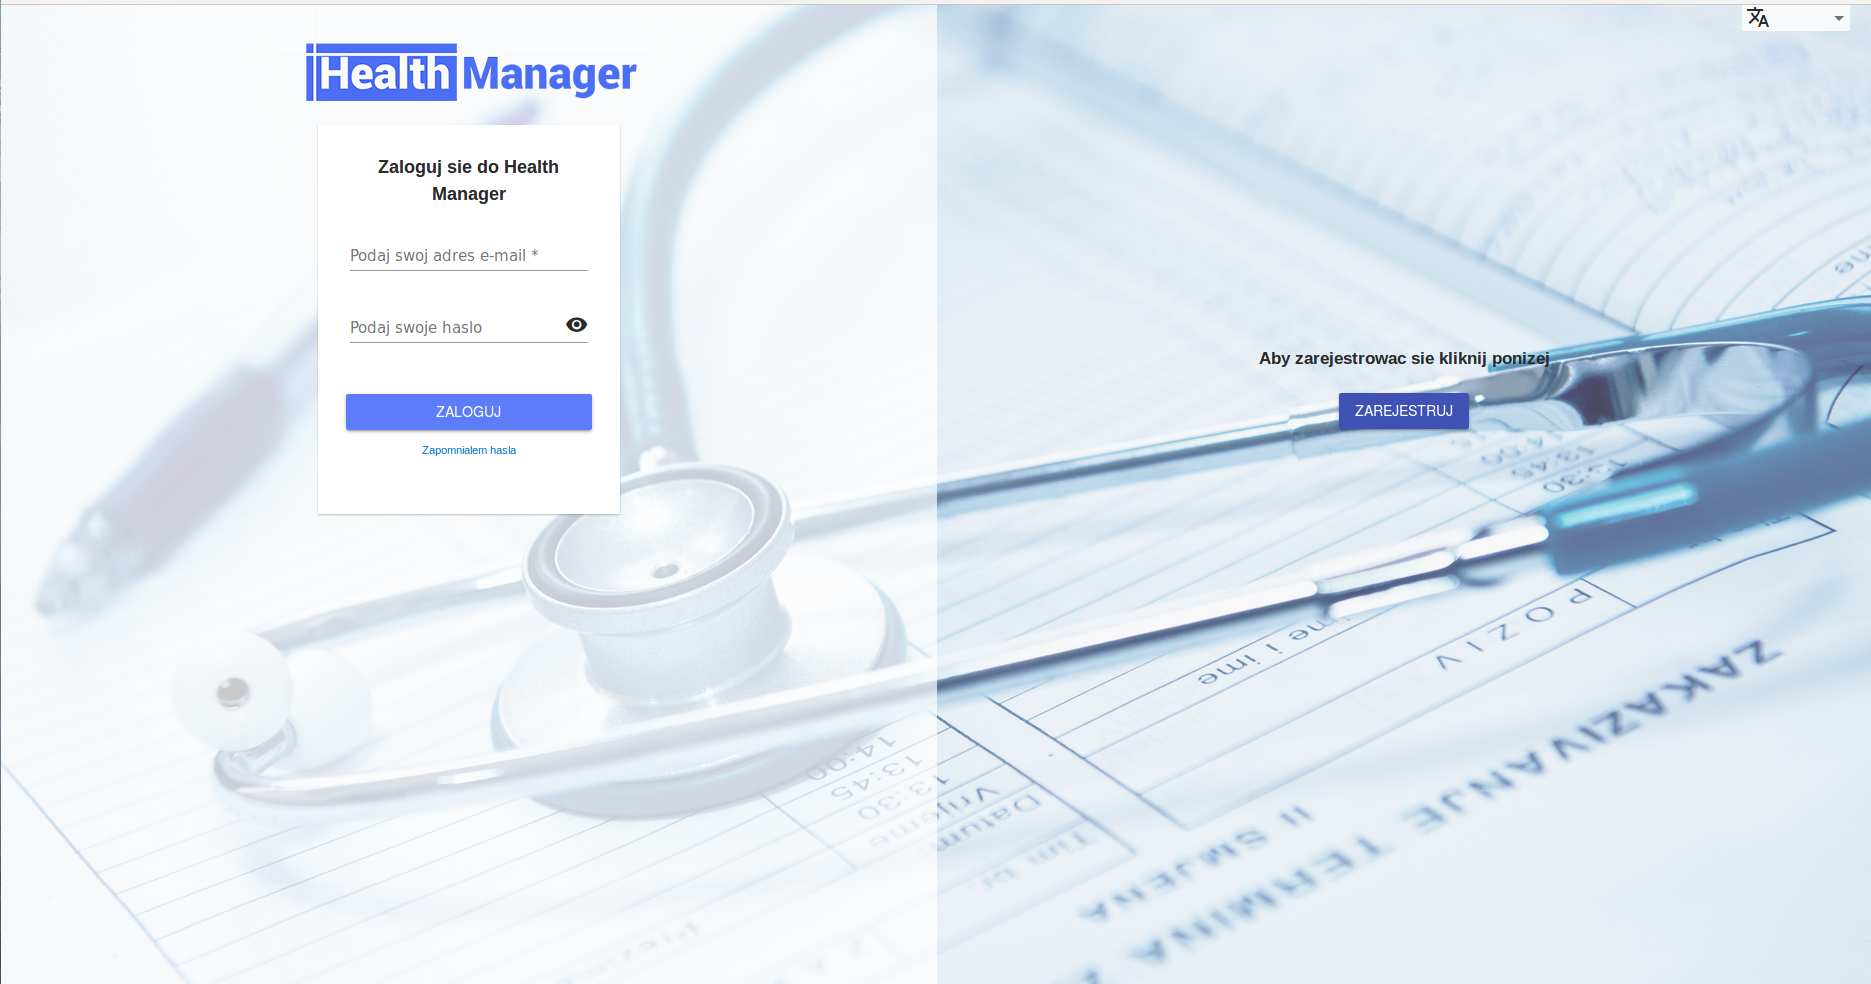
\includegraphics[width=0.7\textwidth]{gui-loginpage}
        \caption{Strona logowania}
    \end{figure}
    Po zalogowaniu użytkownik zostaje przeniesiony na pulpit
    \begin{figure}[H]
        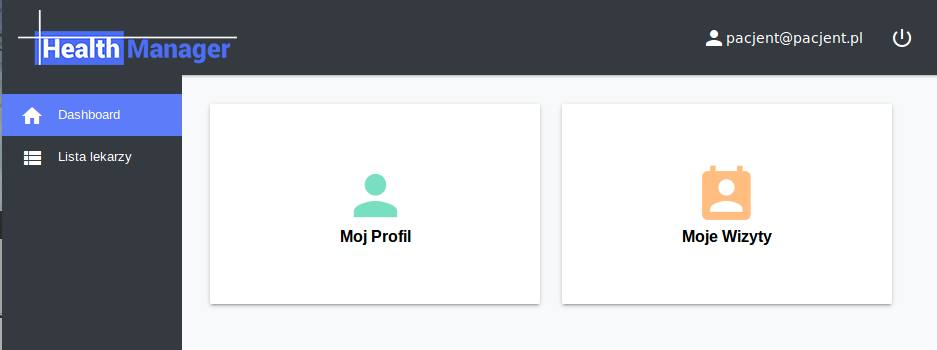
\includegraphics[width=0.7\textwidth]{gui-patient-dashboard}
        \caption{Pulpit pacjenta}
    \end{figure}
        
    }
    \paragraph{Moje wizyty}{Lista umówionych wizyt, pozwala wyświetlić wizyty przyszłe i już odbyte w zależności od wybranego przedziału czasowego. Dostarczane informacje:
    \begin{itemize}
        \item Termin wizyty,
        \item Imię i nazwisko lekarza,
        \item Numer gabinetu,
        \item odnośnik do szczegółowych informacji na temat wizyty.
    \end{itemize}
    %%TODO WSTAWIĆ NOWY OBRAZEK JAK BĘDZIE NAPRAWIONY BUG ŻE PACJENT NIE MOŻE OTRZYMAĆ INFO O SAMYM SOBIE
        \begin{figure}[H]
        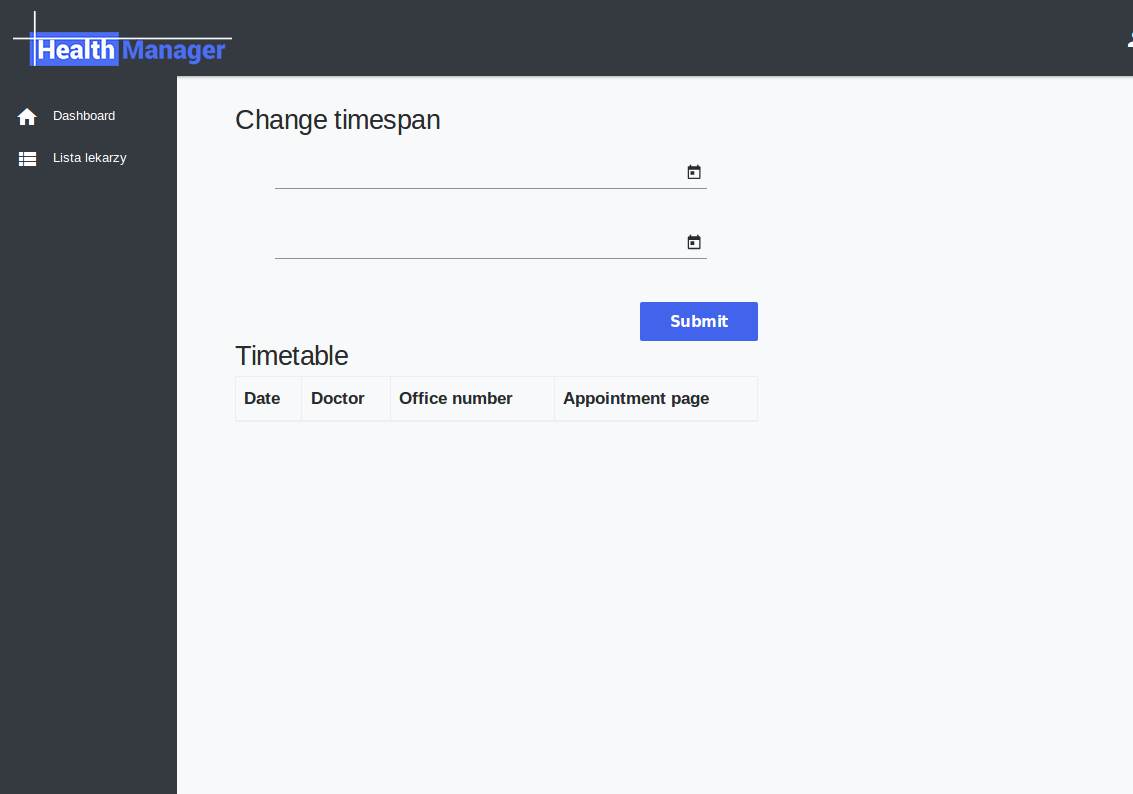
\includegraphics[width=0.7\textwidth]{gui-patient-my-visits}
        \caption{Lista umówionych wizyt pacjenta}
    \end{figure}    
    }
    \paragraph{Lista lekarzy} pozwala na umówienie się na wizytę z konkretnym lekarzem
    \begin{figure}[H]
        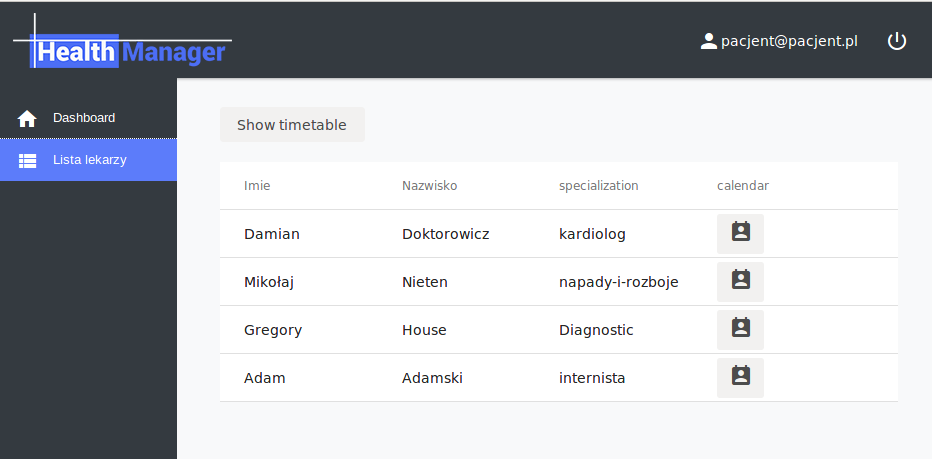
\includegraphics[width=0.7\textwidth]{gui-doctor-list}
        \caption{Lista lekarzy}
    \end{figure}
    Aby zobaczyć dostępne terminy dla danego lekarza należy kliknąć ikonkę kalendarzyka w wierszu zawierającym nazwisko danego lekarza
    \paragraph{Kalendarz lekarza}{ pozwala zobaczyć
    \begin{itemize}
        \item Dostępne terminy wizyt - oznaczone kolorem niebieskim,
        \item Umówione wizyty - oznaczone kolorem czerwonym.
    \end{itemize}
    
    
    \begin{figure}[H]
        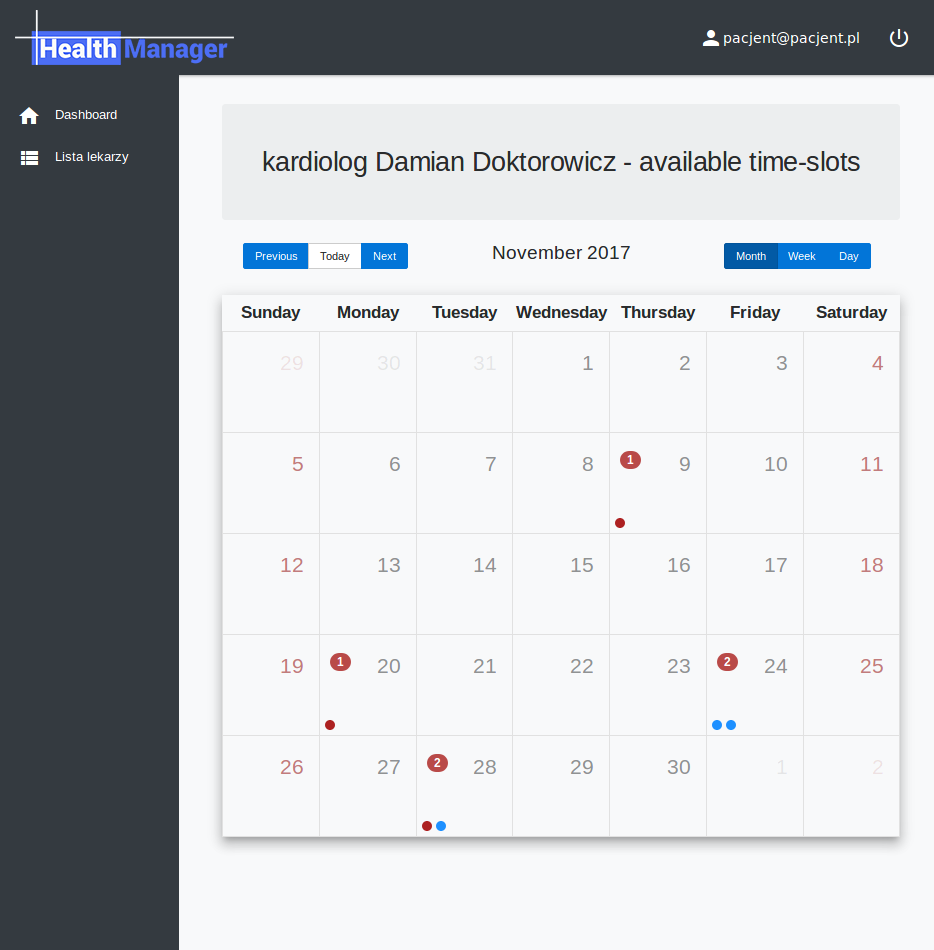
\includegraphics[width=0.7\textwidth]{gui-calendar-patient-month}
        \caption{Kalendarz lekarza - widok miesiąca}
    \end{figure}    
    \begin{figure}[H]
        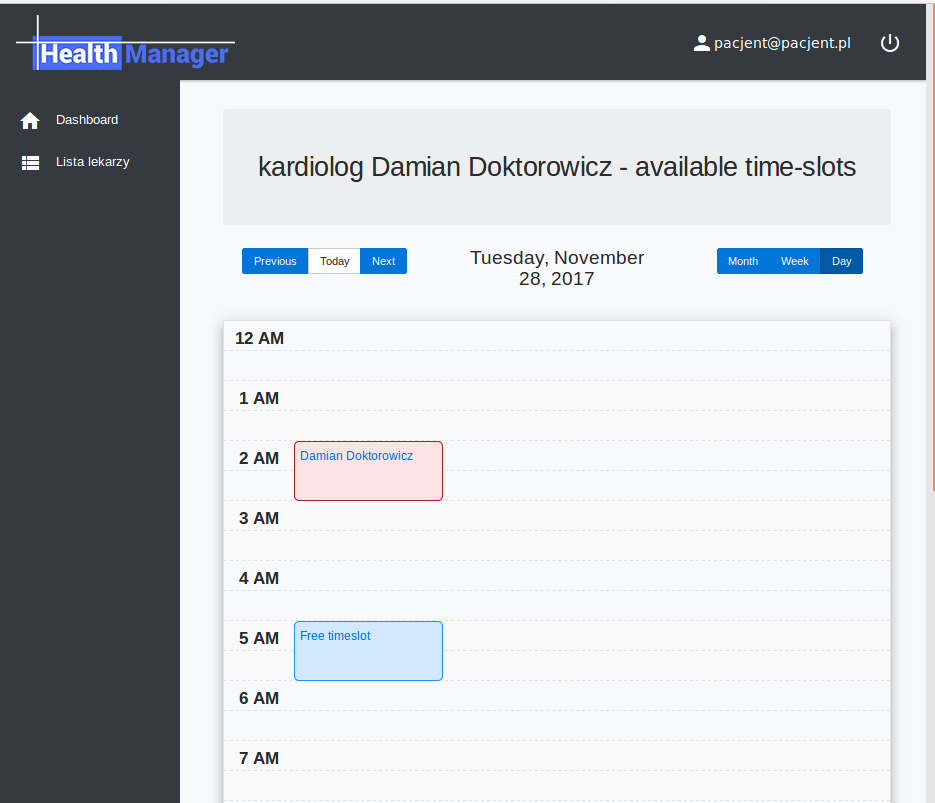
\includegraphics[width=0.7\textwidth]{gui-calendar-patient-day}
        \caption{Kalendarz lekarza - widok dnia}
    \end{figure}    
    }
    \paragraph{Zapis na wizytę}{  - Po kliknięciu na dostępny (oznaczony kolorem niebieskim) termin w widoku kalendarza można się na umówić na wizytę klikając zielony przycisk \emph{Zapisz}. Powód wizyty (bądź inną informację do przekazania lekarzowi) można wpisać w pole \emph{Powód wizyty}
    \begin{figure}[H]
        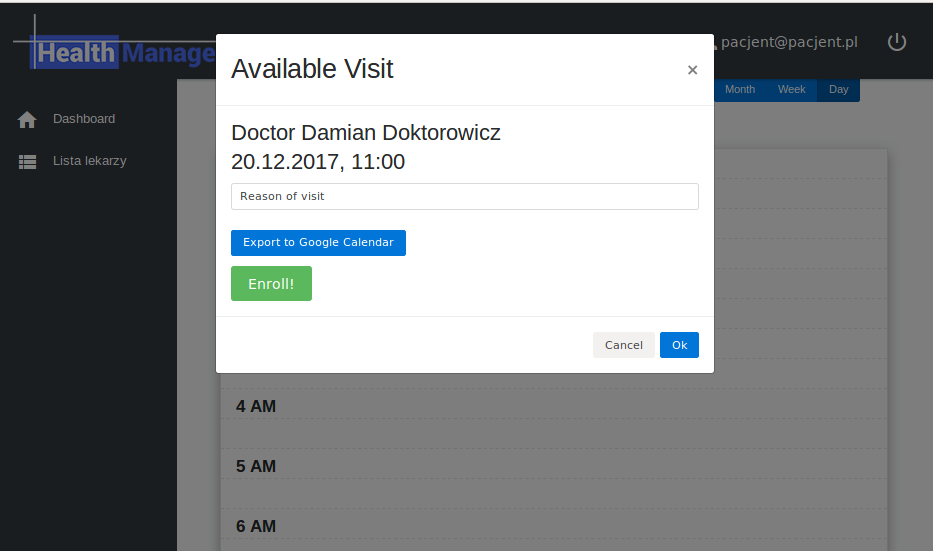
\includegraphics[width=0.7\textwidth]{gui-patient-unenrolled-visit-window}
        \caption{Okno zapisu na wizytę}
    \end{figure}    
    }
    \paragraph{Odwołanie wizyty}{- Po kliknięciu na planowany (oznaczony kolorem czerwonym) termin w widoku kalendarza można odwołać wizytę klikając \emph{Odwołaj}        
        \begin{figure}[H]
        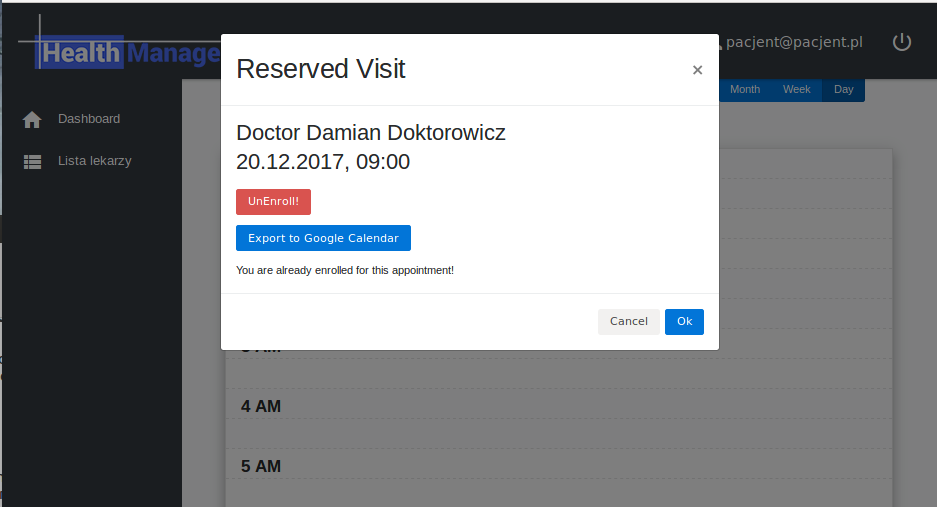
\includegraphics[width=0.7\textwidth]{gui-patient-enrolled-visit-window}
        \caption{Okno zapisanej wizyty}
        \end{figure}  
    }
    \paragraph{Eksport do kalendarza Google.}{ W oknie zapisanej wizyty i oknie zapisu można wyeksportować termin do kalendarza Google klikając \emph{Eksportuj do kalendarza Google}.
    \begin{enumerate},
      \item Kliknij \emph{Eksportuj do kalendarza Google}
      \item W otorzonym okienku uzupełnij swoje dane logowania do konta Google.
    \end{enumerate}
       \begin{figure}[H]
        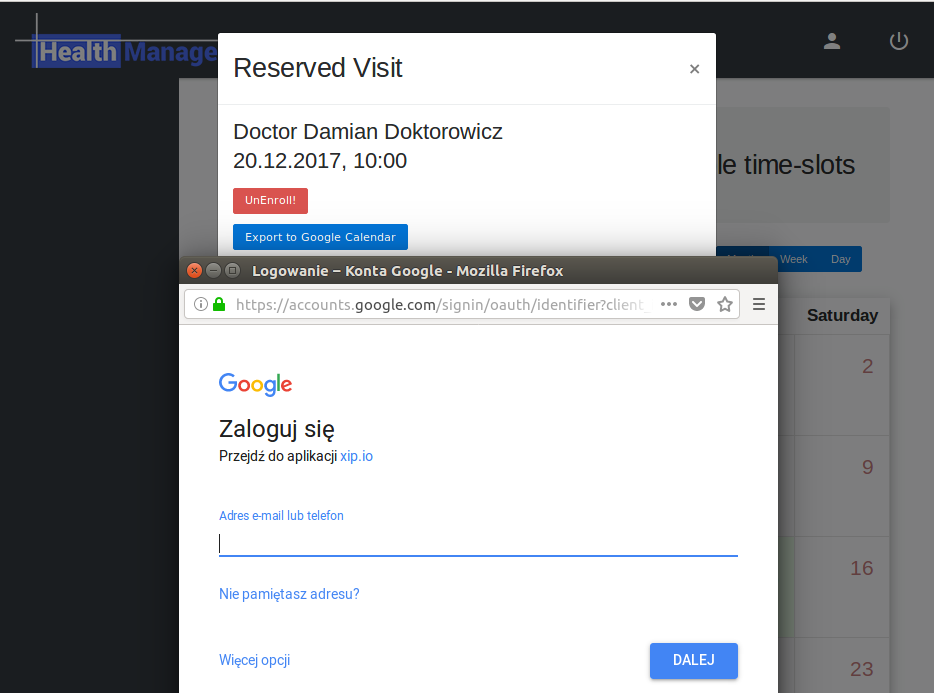
\includegraphics[width=0.7\textwidth]{gui-google-export}
        \caption{Eksport do kalendarza Google}
        \end{figure}  
    }
\subsubsection{Lekarz}
Przewodnik lekarza.
    \paragraph{Logowanie}{
      \begin{enumerate}
          \item Za pomocą przeglądarki internetowej połącz się z serwerem udostępniającym usługę,
          \item Wpisz swój adres e-mail oraz swoje hasło.
      \end{enumerate}
      \begin{figure}[H]
          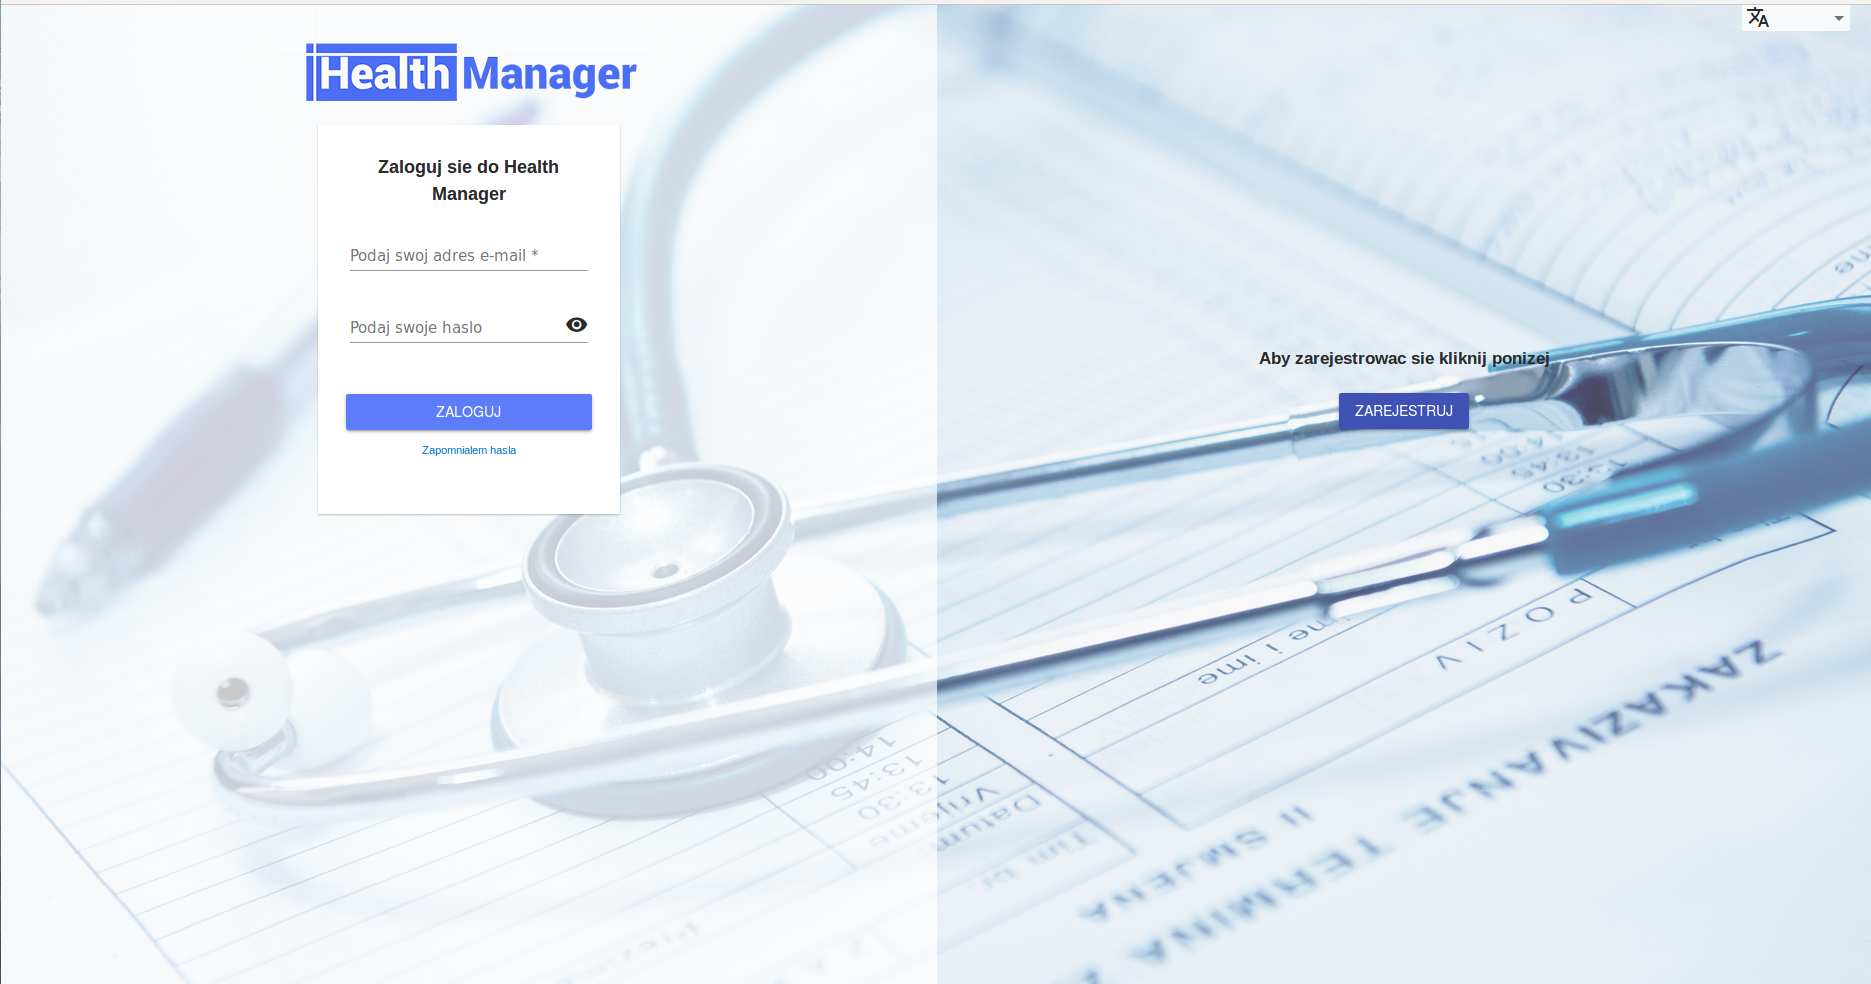
\includegraphics[width=0.7\textwidth]{gui-loginpage}
          \caption{Strona logowania}
      \end{figure}
    }
    \paragraph{Pulpit.}{Po zalogowaniu lekarz przenoszony jest na pulpit
      \begin{figure}[H]
          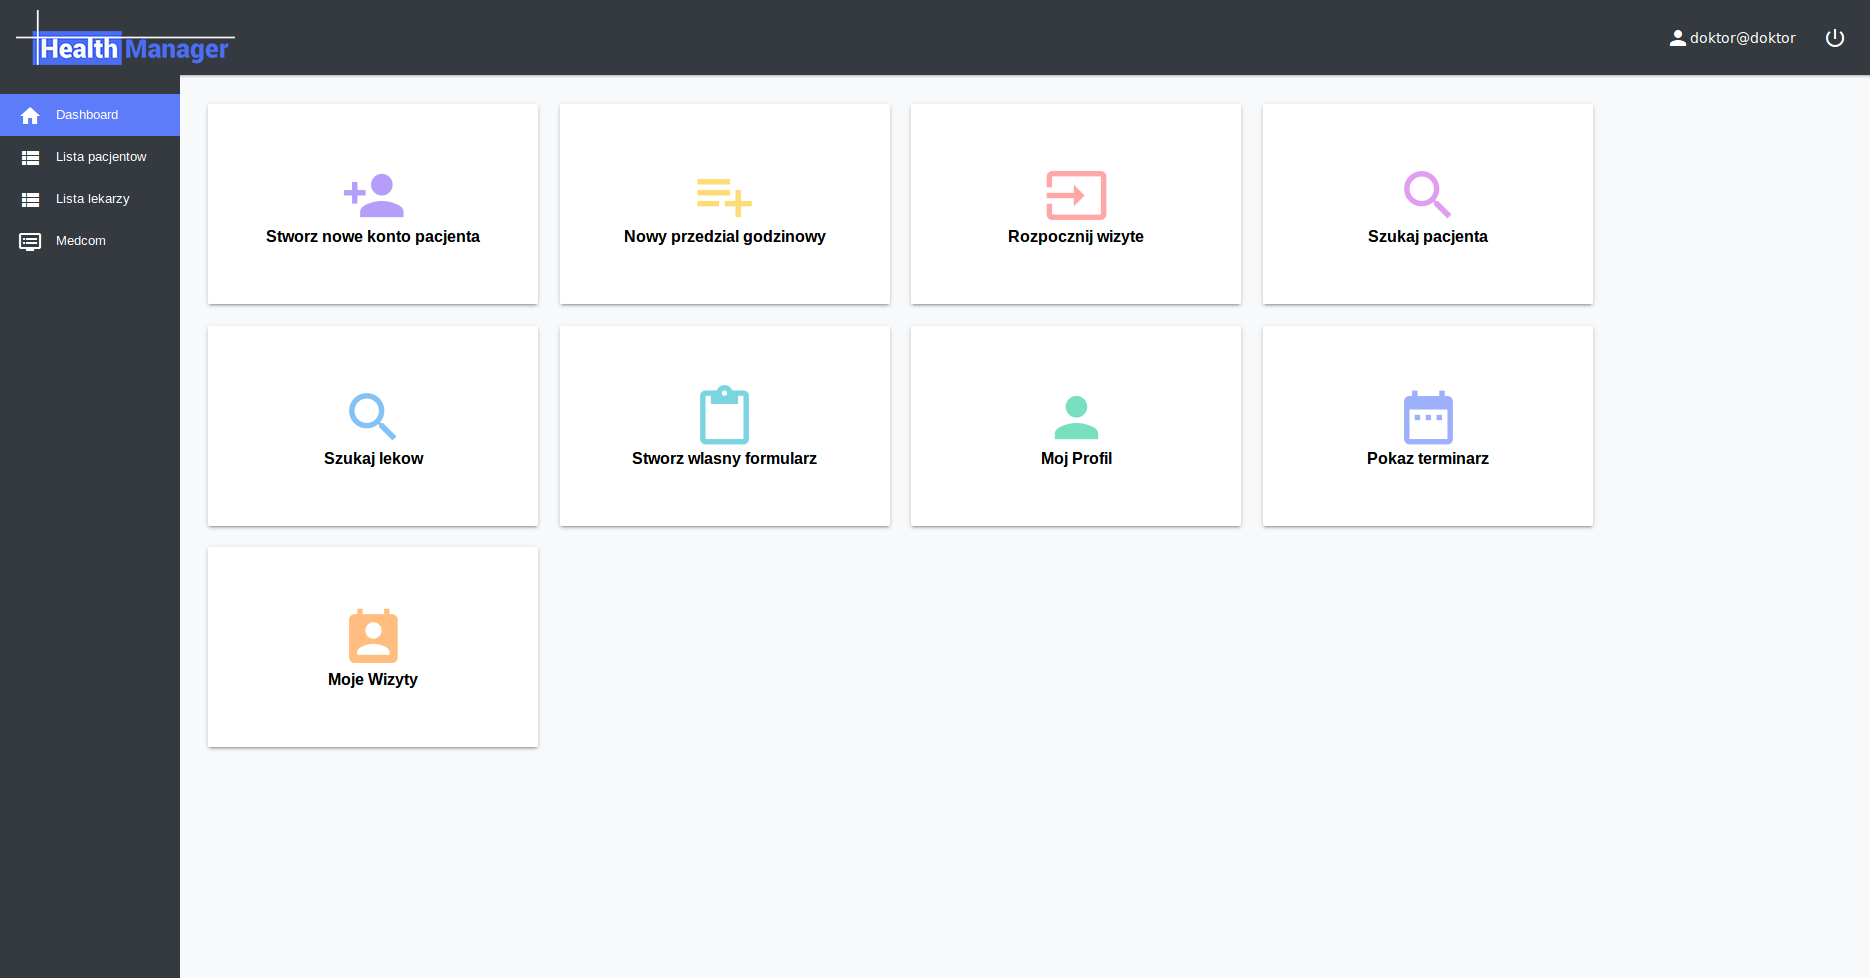
\includegraphics[width=0.7\textwidth]{gui-doc-dashboard}
          \caption{Pulpit lekarza}
      \end{figure} 
    }
    \paragraph{Dodawanie pacjenta}{
        Należy kliknąć w kafelek \emph{Dodaj pacjenta} na pulpicie i wypełnić formularz
        \begin{figure}[H]
          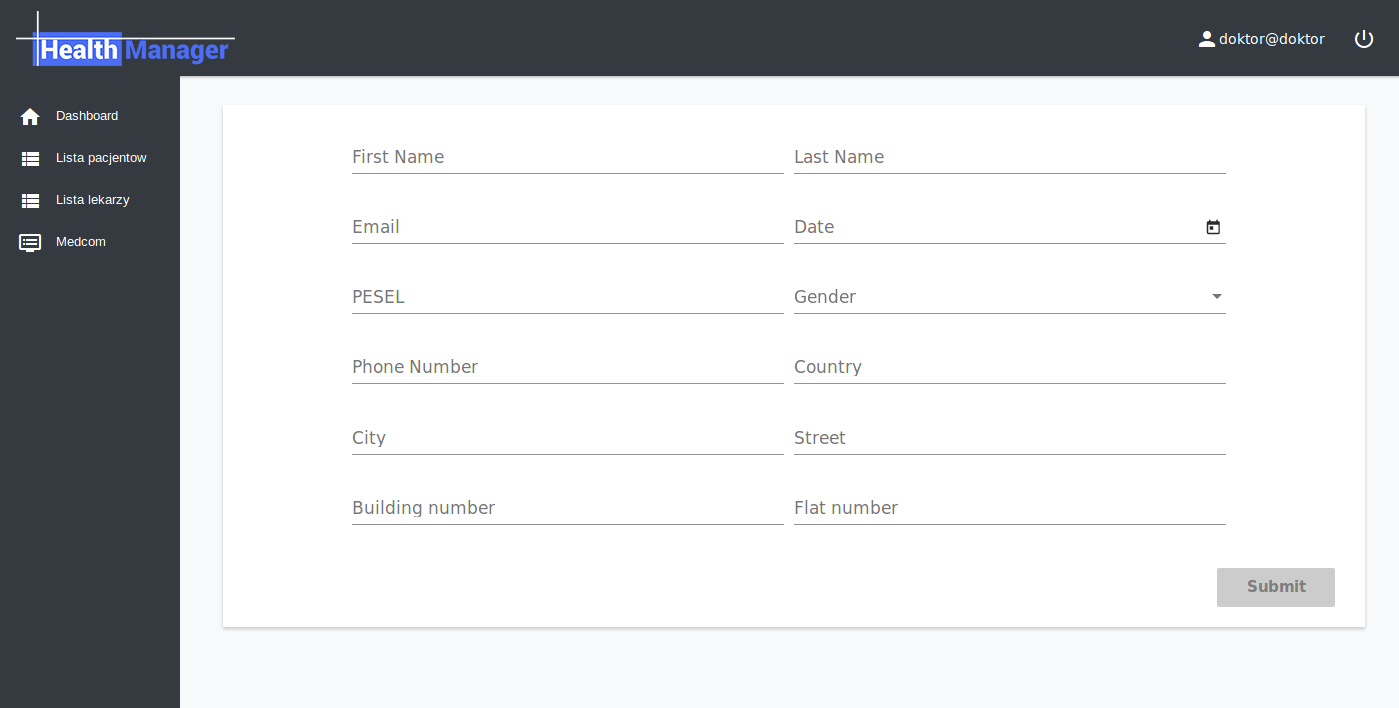
\includegraphics[width=0.7\textwidth]{gui-add-patient}
          \caption{Dodawanie pacjenta}
        \end{figure}     
    }
    \paragraph{Dodawanie dostępnego terminu}{
        Należy kliknąć w kafelek \emph{Dodaj nowy przedział godzinowy} na pulpicie i wypełnić formularz \\
        Wymagane dane:
        \begin{itemize}
            \item Wybierz lekarza - lekarz do którego będzie przypisany termin,
            \item Data - data,
            \item Godzina rozpoczęcia,
            \item Godzina zakończenia,
            \item Pozwól na samo-zapis - określa czy na termin pacjenci mogą rejestrować się samodzielnie czy tylko przez recepcję.
        \end{itemize}
        Po wypełnieniu wyżej wymienionych danych użytkownik może dodać pojedyńczy wolny termin wizyty. Aby dodać wiele terminów na raz, należy wypełnić pozostałe pola. Można dodać wiele terminów  w jednym dniu oraz ustawić tryb powtarzania tak, żeby dodać wiele terminów w wiele dni.
        \begin{itemize}
            \item Minuty na wizytę - czas pojedyńczej wizyty,
            \item Przerwa między wizytami (każdymi dwoma następującymi po sobie),
            \item Tryb powtarzania \begin{itemize}
                \item Bez powtarzania (domyśle) - dodawanie wielu terminów w jednym dniu,
                \item Codziennie,
                \item Co tydzień,
                \item Od poniedziałku do piątku - Tak jak dodawanie codzienne lecz z wyłączeniem sobót i niedziel;
            \end{itemize}
            \item Data zakończenia - nie dotyczy trybu \emph{Bez powtarzania}.
        \end{itemize}
        \begin{figure}[H]
          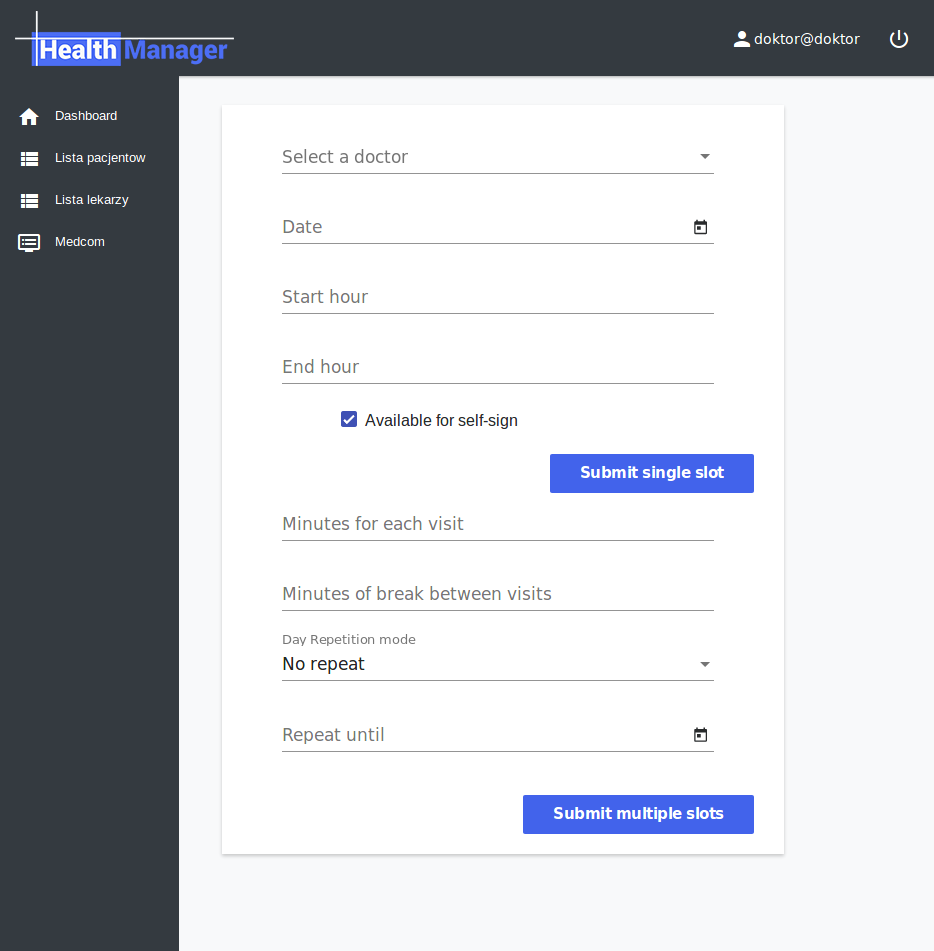
\includegraphics[width=0.7\textwidth]{gui-add-timeslot}
          \caption{Dodawanie dostępnego terminu}
        \end{figure}     
    }
    \paragraph{Grafik}{ Dostępny jest z pulpitu oraz listy lekarzy. Pokazuje wszystkie terminy dla wszystkich lekarzy w zadanym przedziale czasowym
        \begin{figure}[H]
          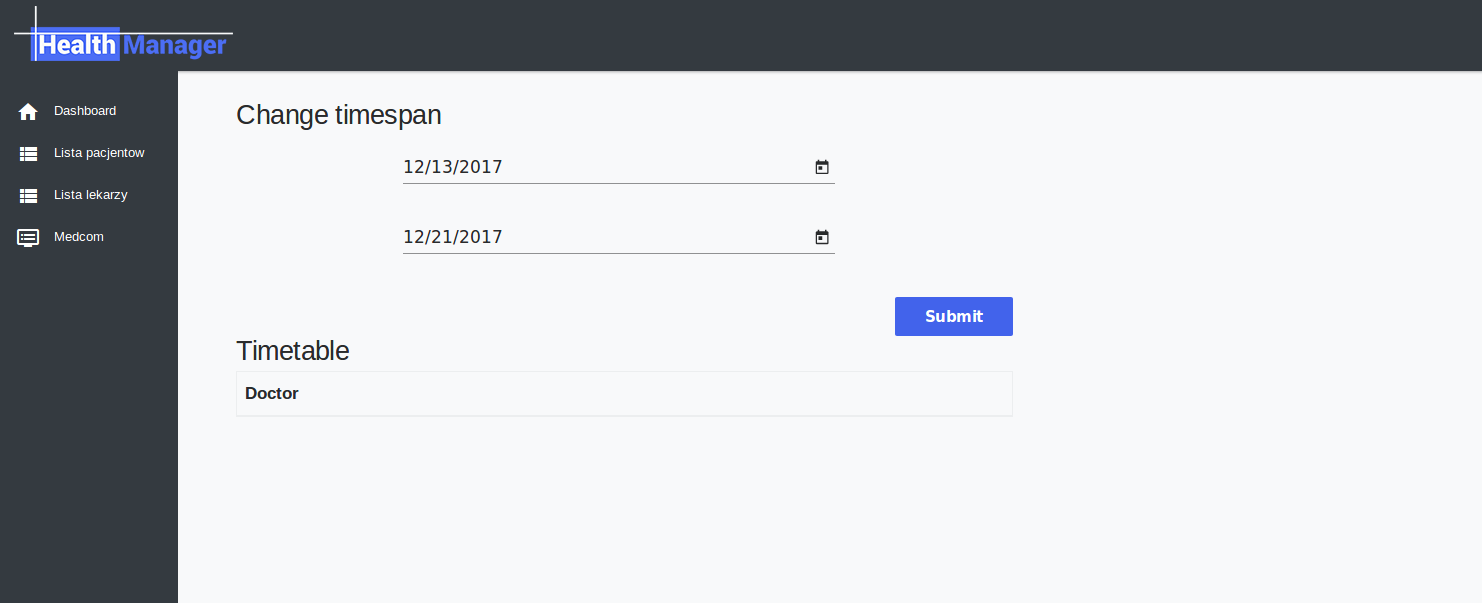
\includegraphics[width=0.7\textwidth]{gui-timetable}
          \caption{Grafik}
        \end{figure}        
    }
    \paragraph{Moje wizyty}{Lista umówionych wizyt, pozwala wyświetlić wizyty przyszłe i już odbyte w zależności od wybranego przedziału czasowego. Dostarczane informacje:
    \begin{itemize}
        \item Termin wizyty,
        \item Imię i nazwisko pacjenta,
        \item Priorytet,
        \item Powód wizyty (wypełniany przez pacjenta przy zapisie),
        \item Numer gabinetu,
        \item odnośnik do szczegółowych informacji na temat wizyty.
    \end{itemize}
        \begin{figure}[H]
        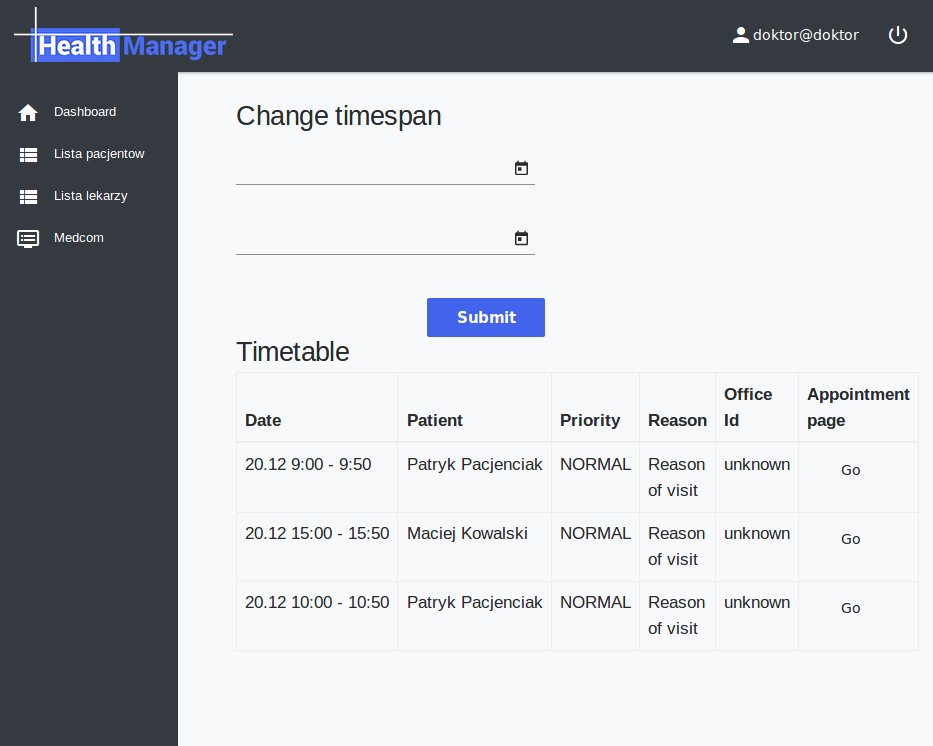
\includegraphics[width=0.7\textwidth]{gui-doc-myvisits}
        \caption{Lista umówionych wizyt lekarza}
        \end{figure}    
    }
    \paragraph{Widok kalendarza} { Lekarz widzi w kalendarzu swoje wolne terminy (zaznaczone na niebiesko) i zajęte swoje terminy (zaznaczone na czerwono) \\
    Aby zobaczyć szczegóły dotyczące terminu należy na niego kliknąć
        \begin{figure}[H]
        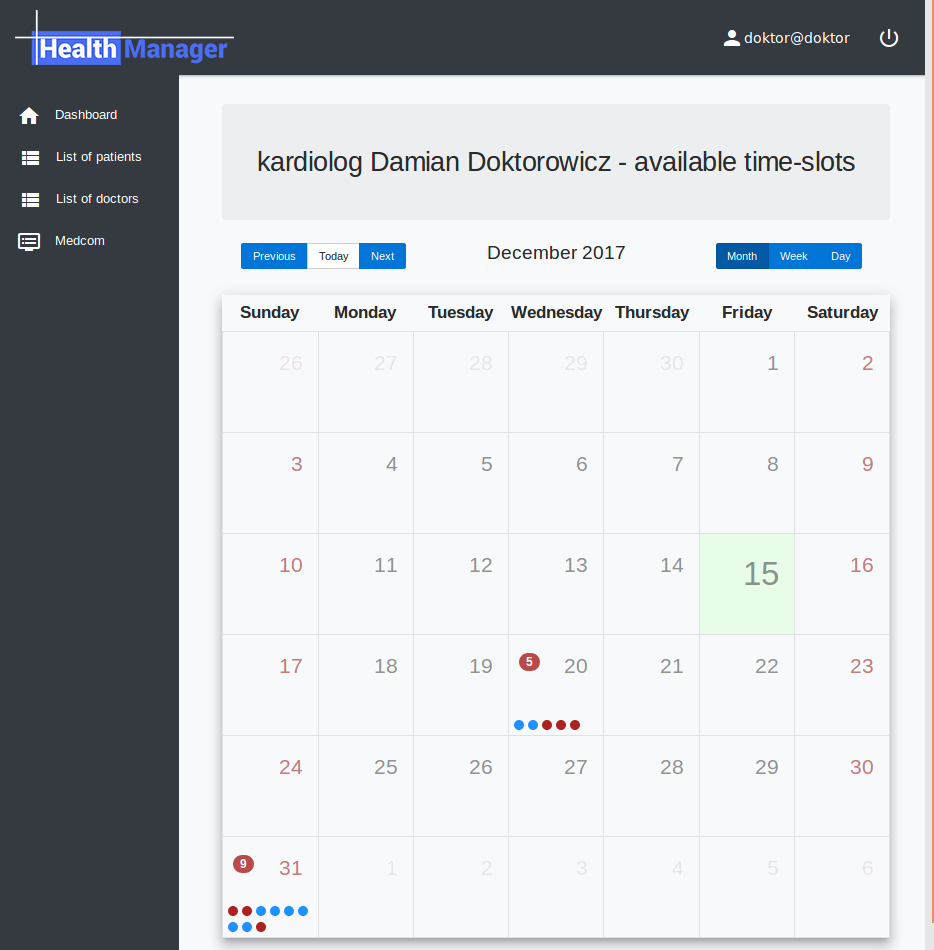
\includegraphics[width=0.7\textwidth]{gui-doc-cal}
        \caption{Kalendarz lekarza}
        \end{figure}  
        }
    \paragraph{Umawianie pacjenta na wizytę}{
    Lekarz może umówić dowolnego pacjenta na wizytę klikając na swój wolny termin i wybierając nazwisko pacjenta z listy
        \begin{figure}[H]
        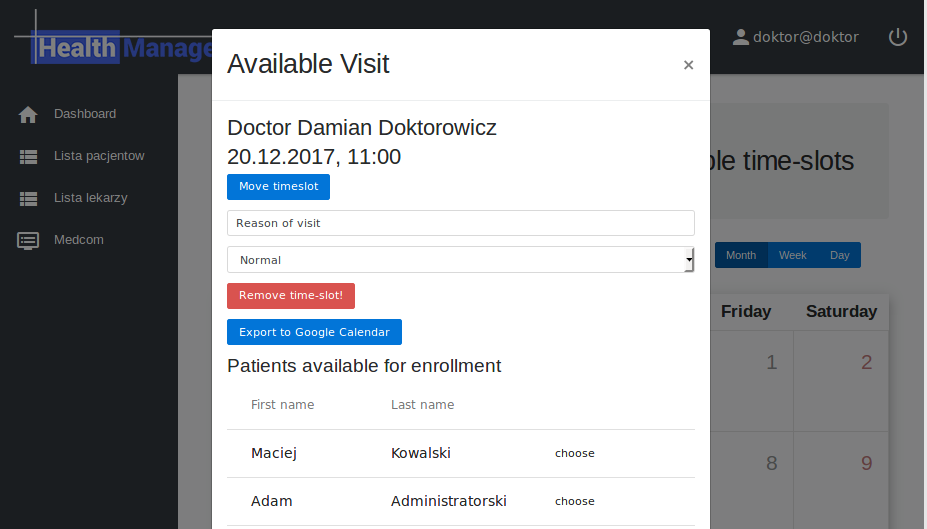
\includegraphics[width=0.7\textwidth]{gui-doc-unenrolled}
        \caption{Zapisywanie pacjenta na wizytę}
        \end{figure}  
    }
     \paragraph{Przeglądanie danych pacjenta zapisanego na wizytę}{
        \begin{enumerate}
          \item Wybierz termin w kalendarzu,
          \item Klinkij na nazwisko pacjenta.
        \end{enumerate}
        \begin{figure}[H]
        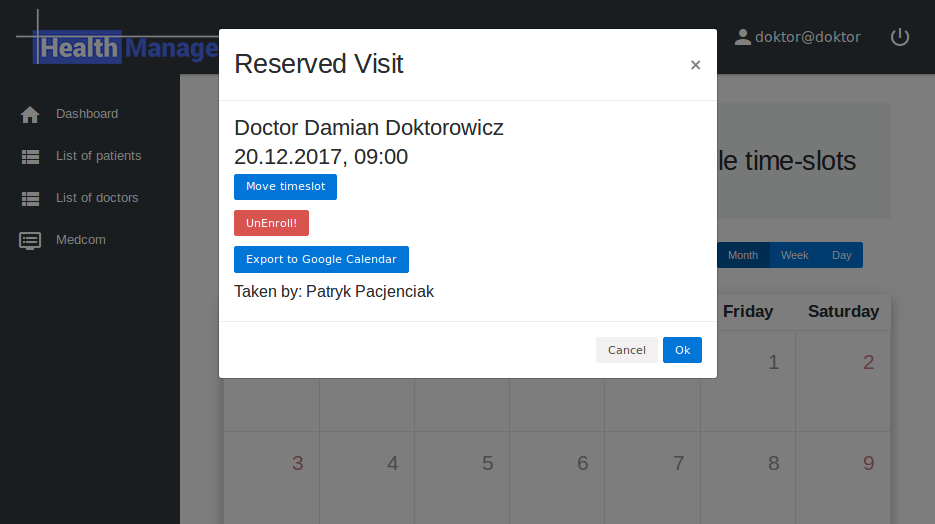
\includegraphics[width=0.7\textwidth]{gui-doc-enrolled}
        \caption{Odwołanie terminu}
        \end{figure}  
    }
     \paragraph{Odwołanie wizyty}{
     Lekarz może odwołać umówioną wizytę wybierając zajęty termin i klikając \emph{Odwołaj wizytę}
        \begin{figure}[H]
        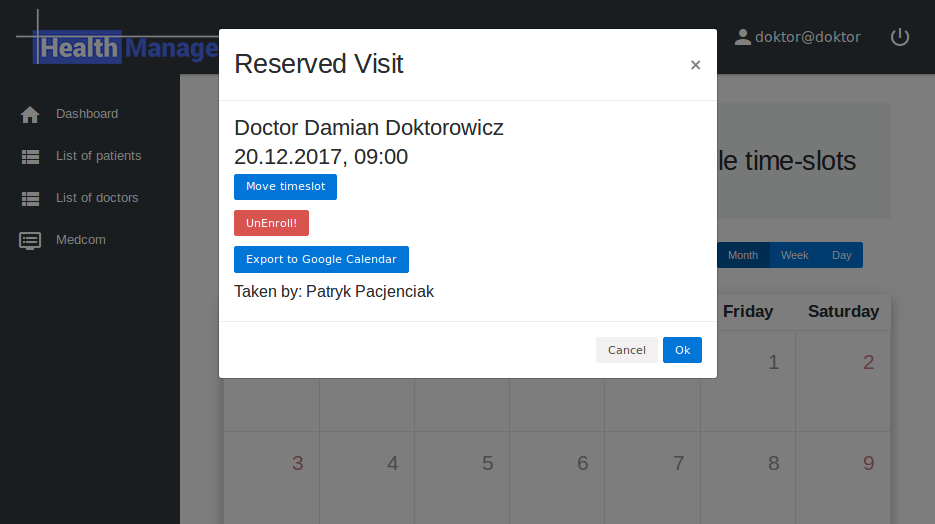
\includegraphics[width=0.7\textwidth]{gui-doc-enrolled}
        \caption{Odwołanie terminu}
        \end{figure}  
    }
    \paragraph{Usuwanie terminu}{
    Lekarz może usunąć swój wolny termin wybierając go w kalendarzu i klikając \emph{Usuń termin}
        \begin{figure}[H]
        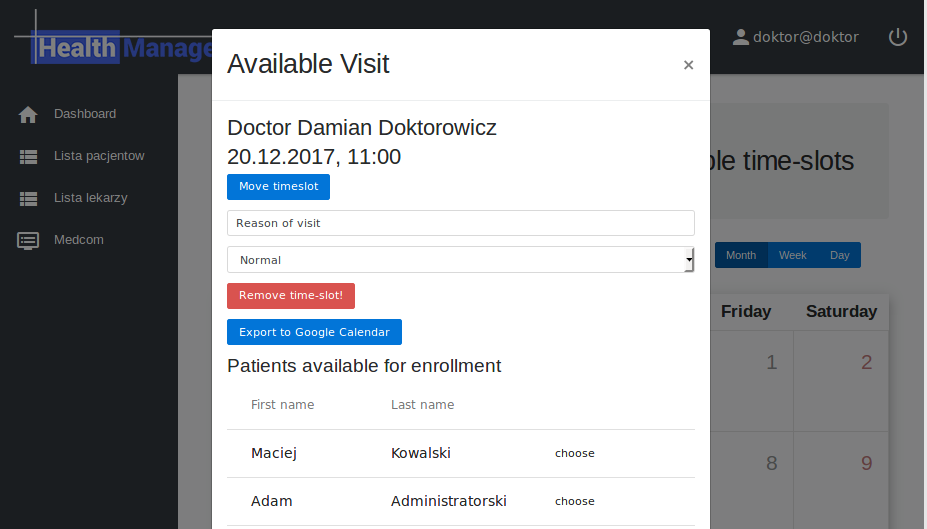
\includegraphics[width=0.7\textwidth]{gui-doc-unenrolled}
        \caption{Usuwanie terminu}
        \end{figure}  
    }
    \paragraph{Przesunięcie terminu}{
    Lekarz może przesunąć dowolny termin (zajęty bądź nie)
    \begin{enumerate}
      \item Wybierz termin w kalendarzu,
      \item Kliknij \emph{Przenieś termin},
      \item Wybierz nową datę rozpoczęcia i zakończenia wizyty,
      \item Kliknij \emph{Zapisz}.
    \end{enumerate}
        \begin{figure}[H]
        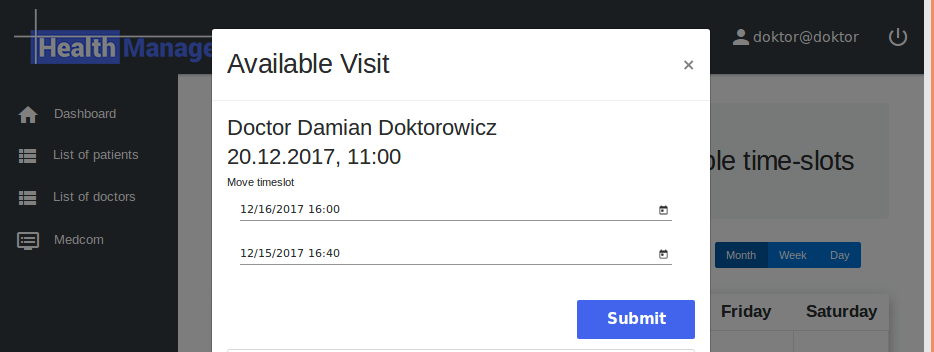
\includegraphics[width=0.7\textwidth]{gui-doc-moveslot}
        \caption{Przesuwanie terminu}
        \end{figure}  
    }
    \paragraph{Eksport do kalendarza Google.}{ W oknie zapisanej wizyty i oknie zapisu można wyeksportować termin do kalendarza Google klikając \emph{Eksportuj do kalendarza Google}.
    \begin{enumerate}
      \item Kliknij \emph{Eksportuj do kalendarza Google},
      \item W otorzonym okienku uzupełnij swoje dane logowania do konta Google.
    \end{enumerate}
       \begin{figure}[H]
        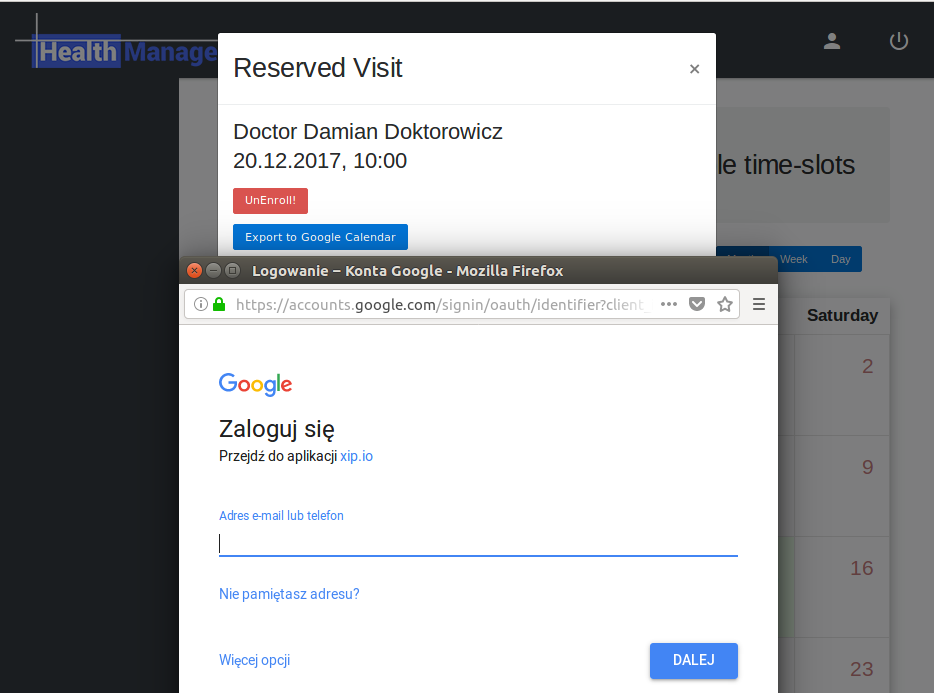
\includegraphics[width=0.7\textwidth]{gui-google-export}
        \caption{Eksport do kalendarza Google}
        \end{figure}  
    }
\subsubsection{Recepcjonistka}
Przewodnik recepcjonistki.
    \paragraph{Logowanie}{
      \begin{enumerate}
          \item Za pomocą przeglądarki internetowej połącz się z serwerem udostępniającym usługę,
          \item Wpisz swój adres e-mail oraz swoje hasło.
      \end{enumerate}
      \begin{figure}[H]
          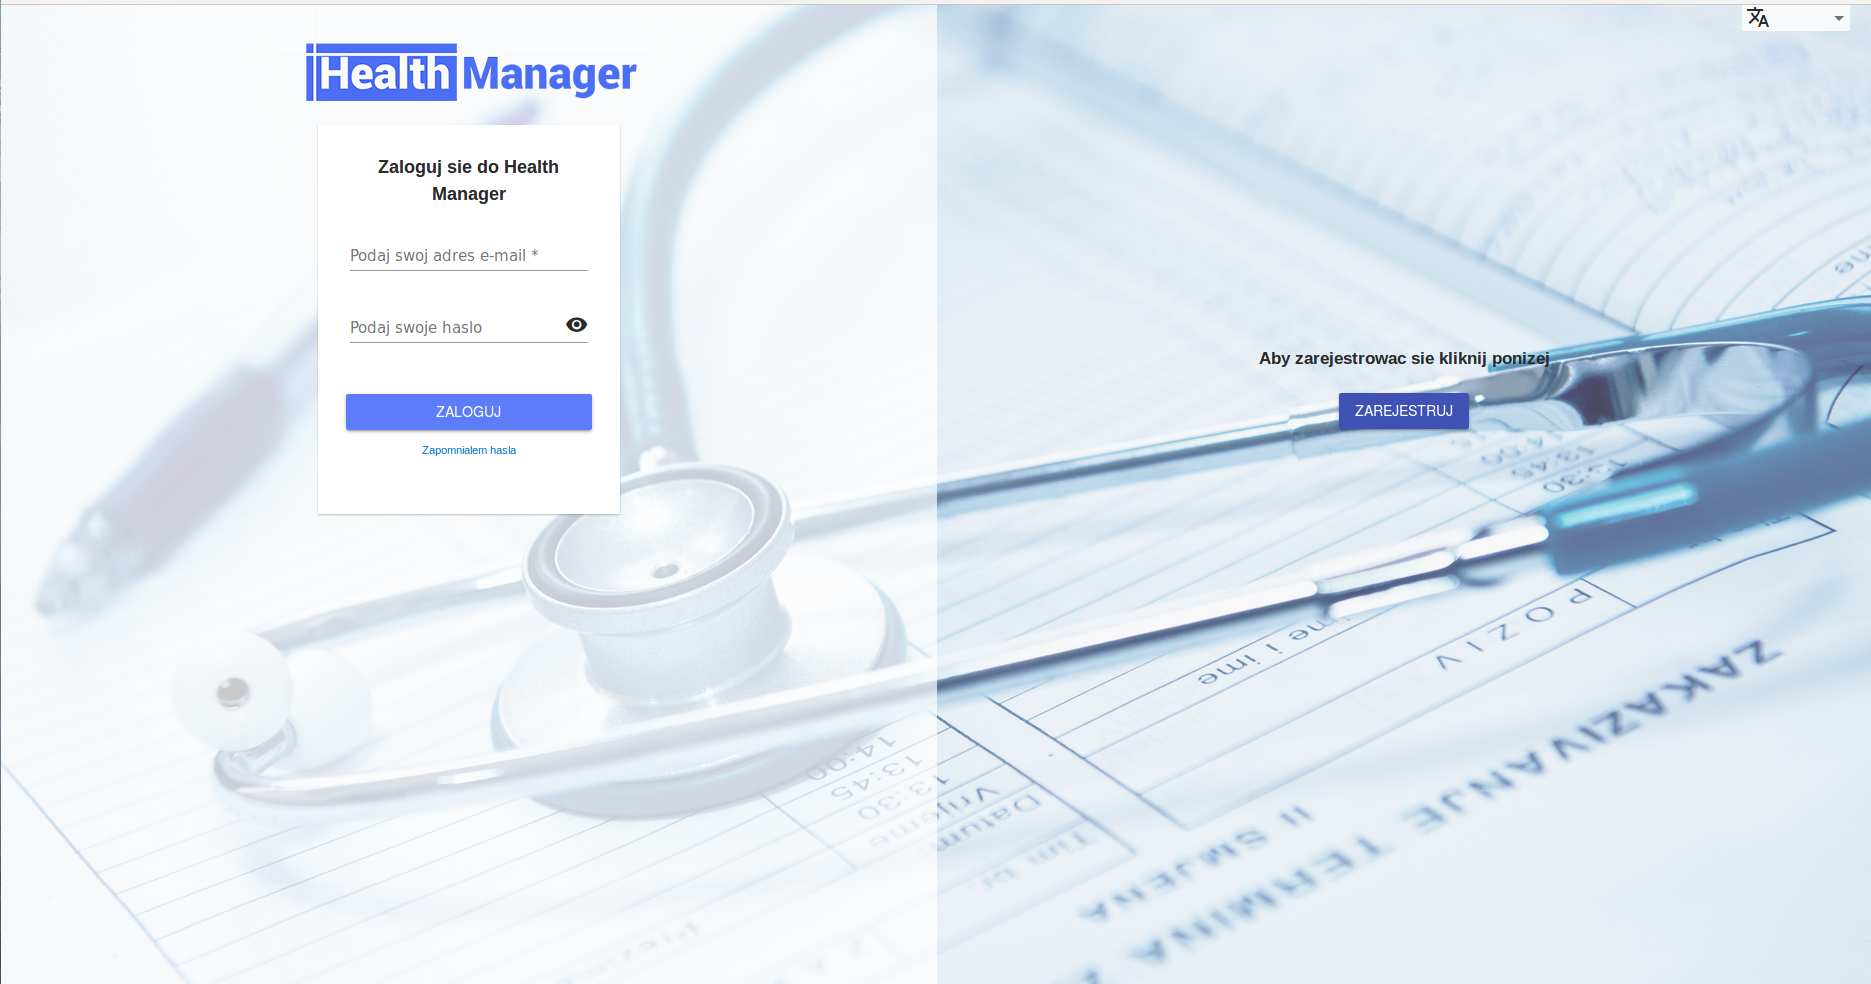
\includegraphics[width=0.7\textwidth]{gui-loginpage}
          \caption{Strona logowania}
      \end{figure}
    }
    \paragraph{Dodawanie pacjenta}{
        Należy kliknąć w kafelek \emph{Dodaj pacjenta} na pulpicie i wypełnić formularz
        \begin{figure}[H]
          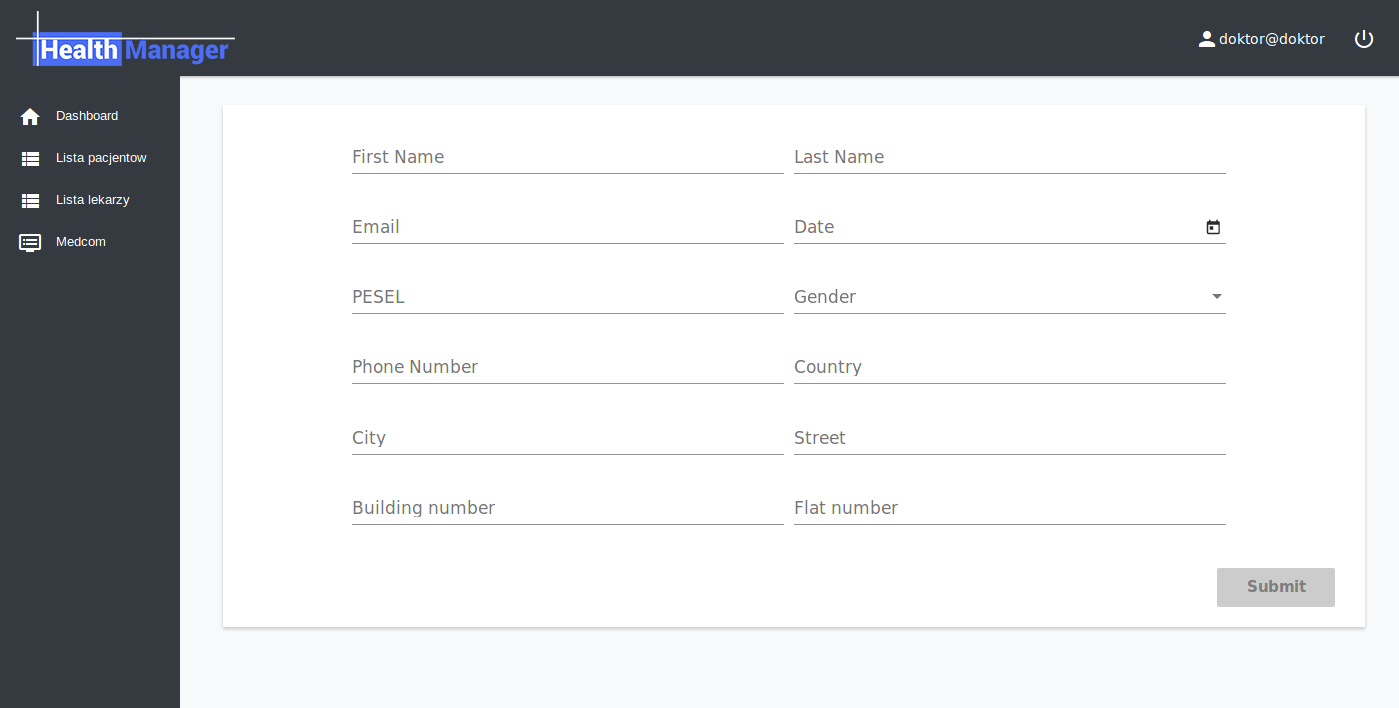
\includegraphics[width=0.7\textwidth]{gui-add-patient}
          \caption{Dodawanie pacjenta}
        \end{figure}     
    }
    \paragraph{Dodawanie lekarza}{
        Należy kliknąć w kafelek \emph{Dodaj lekarza} na pulpicie i wypełnić formularz
        \begin{figure}[H]
          \includegraphics[width=0.7\textwidth]{gui-add-doctor}
          \caption{Dodawanie lekarza}
        \end{figure}     
    }
    \paragraph{Zmiana terminu wizyty}{
      \begin{enumerate}
        \item Wybierz termin w kalendarzu,
        \item Kliknij \emph{Przenieś termin},
        \item Wybierz nowego lekarz obsługującego wizytę,
        \item Wybierz nową datę rozpoczęcia i zakończenia wizyty,
        \item Kliknij \emph{Zapisz}.
      \end{enumerate}
        \begin{figure}[H]
        \includegraphics[width=0.7\textwidth]{gui-recep-moveslot}
        \caption{Zmiana terminu wizyty}
        \end{figure} 
    }
    \paragraph{Rejestracja pacjenta}{
       \begin{itemize}
           \item Najpierw wybór pacjenta - potem wybór lekarza
           \begin{enumerate}
             \item Wybierz \emph{Listę pacjentów} z menu po lewej,
             \item Kliknij \emph{Rejestruj wizytę} przy wybranym pacjencie
               \begin{figure}[H]
               \includegraphics[width=0.7\textwidth]{gui-recep-patientlist}
               \caption{Lista pacjentów}
               \end{figure},
             \item Wybierz lekarza z lity
               \begin{figure}[H]
               \includegraphics[width=0.7\textwidth]{gui-recep-register-for-patient}
               \caption{Wybór lekarza}
               \end{figure} ,
             \item Wybierz termin
               \begin{figure}[H]
               \includegraphics[width=0.7\textwidth]{gui-recep-reg-pat-cal}
               \caption{Wybór terminu}
               \end{figure}  ,
             \item Potwierdź klikając \emph{Zapisz}
               \begin{figure}[H]
               \includegraphics[width=0.7\textwidth]{gui-recep-reg-pat-window}
               \caption{Zatwierdzenie wyboru}
               \end{figure}.            
           \end{enumerate},
           \item Najpierw wybór lekarza - potem wybór pacjenta
             \begin{enumerate}
             \item Kliknij \emph{Lista lekarzy} z menu po lewej,
             \item Wybierz lekarza z listy
                \begin{figure}[H]
                 \includegraphics[width=0.7\textwidth]{gui-doctor-list}
                 \caption{Lista lekarzy}
                 \end{figure},  
             \item Wybierz wolny termin
                 \begin{figure}[H]
                 \includegraphics[width=0.7\textwidth]{gui-doc-cal}
                 \caption{Kalendarz lekarza}
                 \end{figure},  
            \item Wybierz pacjenta z listy
                 \begin{figure}[H]
                 \includegraphics[width=0.7\textwidth]{gui-doc-unenrolled}
                 \caption{Wybór pacjenta}
                 \end{figure}  
             \end{enumerate}.
       \end{itemize}
    }
    \paragraph{Dodawanie dostępnego terminu}{
        Należy kliknąć w kafelek \emph{Dodaj nowy przedział godzinowy} na pulpicie i wypełnić formularz \\
        Wymagane dane:
        \begin{itemize}
            \item Wybierz lekarza - lekarz do którego będzie przypisany termin,
            \item Data - data,
            \item Godzina rozpoczęcia,
            \item Godzina zakończenia,
            \item Pozwól na samo-zapis - określa czy na termin pacjenci mogą rejestrować się samodzielnie czy tylko przez recepcję.
        \end{itemize}
        Po wypełnieniu wyżej wymienionych danych użytkownik może dodać pojedynczy wolny termin wizyty. Aby dodać wiele terminów na raz, należy wypełnić pozostałe pola. Można dodać wiele terminów  w jednym dniu oraz ustawić tryb powtarzania tak, żeby dodać wiele terminów w wiele dni.
        \begin{itemize}
            \item Minuty na wizytę - czas pojedynczej wizyty,
            \item Przerwa między wizytami (każdymi dwoma następującymi po sobie),
            \item Tryb powtarzania \begin{itemize}
                \item Bez powtarzania (domyślne) - dodawanie wielu terminów w jednym dniu,
                \item Codziennie,
                \item Co tydzień,
                \item Od poniedziałku do piątku - Tak jak dodawanie codzienne lecz z wyłączeniem sobót i niedziel;
            \end{itemize}
            \item Data zakończenia - nie dotyczy trybu \emph{Bez powtarzania},
        \end{itemize}
        \begin{figure}[H]
          \includegraphics[width=0.7\textwidth]{gui-add-timeslot}
          \caption{Dodawanie dostępnego terminu}
        \end{figure}     
    }
\newpage
\listoffigures 
\newpage
%%%%% KONIEC %%%%%%
% o ile to mozliwe prosze uzywac odwolan \cite w konkretnych miejscach a nie \nocite



\begin{thebibliography}{9}
\bibitem{rest-doc}
Roy T. Fielding, Richard N. Taylor, \emph{Principled Design of the Modern
Web Architecture}
\\\texttt{http://www.ics.uci.edu/\~{}taylor/documents/2002-REST-TOIT.pdf}

\bibitem{jwt-doc} 
Sebastián Peyrott, JWT Handbook, 
\\\texttt{https://auth0.com/e-books/jwt-handbook}

\bibitem{spring-doc}
Pivotal Software, dokumentacja Springa, 
\\\texttt{https://spring.io/guides}

\bibitem{angular-doc} 
Google, dokumentacja Angulara, 
\\\texttt{https://angular.io/docs}

\bibitem{java-doc} 
Sun Microsystems, Oracle, dokumentacja Javy, 
\\\texttt{https://docs.oracle.com/javase/7/docs/api/}
 
\bibitem{latex-doc} 
Michael Cribbin, Latex tutorial,
\\\texttt{https://www.sharelatex.com/learn/}

\bibitem{stackoverflow} 
Stack Exchange, Inc., praca zbiorowa, zbiór pytań i odpowiedzi,
\\\texttt{https://stackoverflow.com/}

\bibitem{wikipedia} 
Jimmy Wales, praca zbiorowa, encyklopedia
\\\texttt{https://pl.wikipedia.org/}

\end{thebibliography}

%\nocite{artykul2011,ksiazka2011,narzedzie2011,projekt2011}
%\bibliography{bibliografia}

\end{document}
